\documentclass[twoside]{book}

% Packages required by doxygen
\usepackage{fixltx2e}
\usepackage{calc}
\usepackage{doxygen}
\usepackage[export]{adjustbox} % also loads graphicx
\usepackage{graphicx}
\usepackage[utf8]{inputenc}
\usepackage{makeidx}
\usepackage{multicol}
\usepackage{multirow}
\PassOptionsToPackage{warn}{textcomp}
\usepackage{textcomp}
\usepackage[nointegrals]{wasysym}
\usepackage[table]{xcolor}

% Font selection
\usepackage[T1]{fontenc}
\usepackage[scaled=.90]{helvet}
\usepackage{courier}
\usepackage{amssymb}
\usepackage{sectsty}
\renewcommand{\familydefault}{\sfdefault}
\allsectionsfont{%
  \fontseries{bc}\selectfont%
  \color{darkgray}%
}
\renewcommand{\DoxyLabelFont}{%
  \fontseries{bc}\selectfont%
  \color{darkgray}%
}
\newcommand{\+}{\discretionary{\mbox{\scriptsize$\hookleftarrow$}}{}{}}

% Page & text layout
\usepackage{geometry}
\geometry{%
  a4paper,%
  top=2.5cm,%
  bottom=2.5cm,%
  left=2.5cm,%
  right=2.5cm%
}
\tolerance=750
\hfuzz=15pt
\hbadness=750
\setlength{\emergencystretch}{15pt}
\setlength{\parindent}{0cm}
\setlength{\parskip}{3ex plus 2ex minus 2ex}
\makeatletter
\renewcommand{\paragraph}{%
  \@startsection{paragraph}{4}{0ex}{-1.0ex}{1.0ex}{%
    \normalfont\normalsize\bfseries\SS@parafont%
  }%
}
\renewcommand{\subparagraph}{%
  \@startsection{subparagraph}{5}{0ex}{-1.0ex}{1.0ex}{%
    \normalfont\normalsize\bfseries\SS@subparafont%
  }%
}
\makeatother

% Headers & footers
\usepackage{fancyhdr}
\pagestyle{fancyplain}
\fancyhead[LE]{\fancyplain{}{\bfseries\thepage}}
\fancyhead[CE]{\fancyplain{}{}}
\fancyhead[RE]{\fancyplain{}{\bfseries\leftmark}}
\fancyhead[LO]{\fancyplain{}{\bfseries\rightmark}}
\fancyhead[CO]{\fancyplain{}{}}
\fancyhead[RO]{\fancyplain{}{\bfseries\thepage}}
\fancyfoot[LE]{\fancyplain{}{}}
\fancyfoot[CE]{\fancyplain{}{}}
\fancyfoot[RE]{\fancyplain{}{\bfseries\scriptsize Generated by Doxygen }}
\fancyfoot[LO]{\fancyplain{}{\bfseries\scriptsize Generated by Doxygen }}
\fancyfoot[CO]{\fancyplain{}{}}
\fancyfoot[RO]{\fancyplain{}{}}
\renewcommand{\footrulewidth}{0.4pt}
\renewcommand{\chaptermark}[1]{%
  \markboth{#1}{}%
}
\renewcommand{\sectionmark}[1]{%
  \markright{\thesection\ #1}%
}

% Indices & bibliography
\usepackage{natbib}
\usepackage[titles]{tocloft}
\setcounter{tocdepth}{3}
\setcounter{secnumdepth}{5}
\makeindex

% Hyperlinks (required, but should be loaded last)
\usepackage{ifpdf}
\ifpdf
  \usepackage[pdftex,pagebackref=true]{hyperref}
\else
  \usepackage[ps2pdf,pagebackref=true]{hyperref}
\fi
\hypersetup{%
  colorlinks=true,%
  linkcolor=blue,%
  citecolor=blue,%
  unicode%
}

% Custom commands
\newcommand{\clearemptydoublepage}{%
  \newpage{\pagestyle{empty}\cleardoublepage}%
}

\usepackage{caption}
\captionsetup{labelsep=space,justification=centering,font={bf},singlelinecheck=off,skip=4pt,position=top}

%===== C O N T E N T S =====

\begin{document}

% Titlepage & ToC
\hypersetup{pageanchor=false,
             bookmarksnumbered=true,
             pdfencoding=unicode
            }
\pagenumbering{roman}
\begin{titlepage}
\vspace*{7cm}
\begin{center}%
{\Large L\+I\+D\+AR Controller \\[1ex]\large v1.\+0 }\\
\vspace*{1cm}
{\large Generated by Doxygen 1.8.11}\\
\end{center}
\end{titlepage}
\clearemptydoublepage
\tableofcontents
\clearemptydoublepage
\pagenumbering{arabic}
\hypersetup{pageanchor=true}

%--- Begin generated contents ---
\chapter{Namespace Index}
\section{Packages}
Here are the packages with brief descriptions (if available)\+:\begin{DoxyCompactList}
\item\contentsline{section}{\hyperlink{namespace_l_i_d_a_r___controller}{L\+I\+D\+A\+R\+\_\+\+Controller} }{\pageref{namespace_l_i_d_a_r___controller}}{}
\end{DoxyCompactList}

\chapter{Hierarchical Index}
\section{Class Hierarchy}
This inheritance list is sorted roughly, but not completely, alphabetically\+:\begin{DoxyCompactList}
\item \contentsline{section}{L\+I\+D\+A\+R\+\_\+\+Controller.\+D\+AO}{\pageref{class_l_i_d_a_r___controller_1_1_d_a_o}}{}
\item \contentsline{section}{L\+I\+D\+A\+R\+\_\+\+Controller.\+Measurement}{\pageref{class_l_i_d_a_r___controller_1_1_measurement}}{}
\item Window\begin{DoxyCompactList}
\item \contentsline{section}{L\+I\+D\+A\+R\+\_\+\+Controller.\+Main\+Window}{\pageref{class_l_i_d_a_r___controller_1_1_main_window}}{}
\end{DoxyCompactList}
\end{DoxyCompactList}

\chapter{Class Index}
\section{Class List}
Here are the classes, structs, unions and interfaces with brief descriptions\+:\begin{DoxyCompactList}
\item\contentsline{section}{\hyperlink{class_l_i_d_a_r___controller_1_1_d_a_o}{L\+I\+D\+A\+R\+\_\+\+Controller.\+D\+AO} \\*A \char`\"{}data access object\char`\"{} class. This is used to separate the file operations from the G\+UI logic }{\pageref{class_l_i_d_a_r___controller_1_1_d_a_o}}{}
\item\contentsline{section}{\hyperlink{class_l_i_d_a_r___controller_1_1_main_window}{L\+I\+D\+A\+R\+\_\+\+Controller.\+Main\+Window} \\*The application\textquotesingle{}s main form. This class contains all necessary event and exception handlers }{\pageref{class_l_i_d_a_r___controller_1_1_main_window}}{}
\item\contentsline{section}{\hyperlink{class_l_i_d_a_r___controller_1_1_measurement}{L\+I\+D\+A\+R\+\_\+\+Controller.\+Measurement} \\*(Serializable) a measurement }{\pageref{class_l_i_d_a_r___controller_1_1_measurement}}{}
\end{DoxyCompactList}

\chapter{File Index}
\section{File List}
Here is a list of all documented files with brief descriptions\+:\begin{DoxyCompactList}
\item\contentsline{section}{L\+I\+D\+A\+R\+\_\+\+V\+I\+S\+\_\+\+T\+E\+S\+T/\+L\+I\+D\+A\+R\+\_\+\+W\+P\+F\+\_\+\+T\+E\+S\+T/\hyperlink{_d_a_o_8cs}{D\+A\+O.\+cs} \\*Implements the dao class }{\pageref{_d_a_o_8cs}}{}
\item\contentsline{section}{L\+I\+D\+A\+R\+\_\+\+V\+I\+S\+\_\+\+T\+E\+S\+T/\+L\+I\+D\+A\+R\+\_\+\+W\+P\+F\+\_\+\+T\+E\+S\+T/\hyperlink{_main_window_8xaml_8cs}{Main\+Window.\+xaml.\+cs} \\*Implements the main window.\+xaml class. This file contains all G\+UI specific code (Event handler for G\+U\+I-\/elements) }{\pageref{_main_window_8xaml_8cs}}{}
\item\contentsline{section}{L\+I\+D\+A\+R\+\_\+\+V\+I\+S\+\_\+\+T\+E\+S\+T/\+L\+I\+D\+A\+R\+\_\+\+W\+P\+F\+\_\+\+T\+E\+S\+T/\hyperlink{_measurement_8cs}{Measurement.\+cs} \\*Implements the measurement class }{\pageref{_measurement_8cs}}{}
\end{DoxyCompactList}

\chapter{Namespace Documentation}
\hypertarget{namespace_l_i_d_a_r___controller}{}\section{L\+I\+D\+A\+R\+\_\+\+Controller Namespace Reference}
\label{namespace_l_i_d_a_r___controller}\index{L\+I\+D\+A\+R\+\_\+\+Controller@{L\+I\+D\+A\+R\+\_\+\+Controller}}
\subsection*{Classes}
\begin{DoxyCompactItemize}
\item 
class \hyperlink{class_l_i_d_a_r___controller_1_1_d_a_o}{D\+AO}
\begin{DoxyCompactList}\small\item\em A \char`\"{}data access object\char`\"{} class. This is used to separate the file operations from the G\+UI logic. \end{DoxyCompactList}\item 
class \hyperlink{class_l_i_d_a_r___controller_1_1_main_window}{Main\+Window}
\begin{DoxyCompactList}\small\item\em The application\textquotesingle{}s main form. This class contains all necessary event and exception handlers. \end{DoxyCompactList}\item 
class \hyperlink{class_l_i_d_a_r___controller_1_1_measurement}{Measurement}
\begin{DoxyCompactList}\small\item\em (Serializable) a measurement. \end{DoxyCompactList}\end{DoxyCompactItemize}

\chapter{Class Documentation}
\hypertarget{class_l_i_d_a_r___controller_1_1_d_a_o}{}\section{L\+I\+D\+A\+R\+\_\+\+Controller.\+D\+AO Class Reference}
\label{class_l_i_d_a_r___controller_1_1_d_a_o}\index{L\+I\+D\+A\+R\+\_\+\+Controller.\+D\+AO@{L\+I\+D\+A\+R\+\_\+\+Controller.\+D\+AO}}


A \char`\"{}data access object\char`\"{} class. This is used to separate the file operations from the G\+UI logic.  


\subsection*{Static Public Member Functions}
\begin{DoxyCompactItemize}
\item 
static List$<$ \hyperlink{class_l_i_d_a_r___controller_1_1_measurement}{Measurement} $>$ \hyperlink{class_l_i_d_a_r___controller_1_1_d_a_o_acfdac277f8f5c97272fafdaecf3252fb}{load\+Measurements} ()
\begin{DoxyCompactList}\small\item\em Loads the measurements from a xml file. First ssk user if he/she wants to load data. If not return null. \end{DoxyCompactList}\item 
static void \hyperlink{class_l_i_d_a_r___controller_1_1_d_a_o_a6ad2697a8c414f60b8076cfdffe433c8}{save\+Measurements} (List$<$ \hyperlink{class_l_i_d_a_r___controller_1_1_measurement}{Measurement} $>$ l)
\begin{DoxyCompactList}\small\item\em Saves the measurements to a xml file. \end{DoxyCompactList}\end{DoxyCompactItemize}


\subsection{Detailed Description}
A \char`\"{}data access object\char`\"{} class. This is used to separate the file operations from the G\+UI logic. 

\begin{DoxyAuthor}{Author}
Alexander Miller (7089316) 
\end{DoxyAuthor}
\begin{DoxyDate}{Date}
22.\+12.\+2015 
\end{DoxyDate}


Definition at line 31 of file D\+A\+O.\+cs.



\subsection{Member Function Documentation}
\index{L\+I\+D\+A\+R\+\_\+\+Controller\+::\+D\+AO@{L\+I\+D\+A\+R\+\_\+\+Controller\+::\+D\+AO}!load\+Measurements@{load\+Measurements}}
\index{load\+Measurements@{load\+Measurements}!L\+I\+D\+A\+R\+\_\+\+Controller\+::\+D\+AO@{L\+I\+D\+A\+R\+\_\+\+Controller\+::\+D\+AO}}
\subsubsection[{\texorpdfstring{load\+Measurements()}{loadMeasurements()}}]{\setlength{\rightskip}{0pt plus 5cm}public static List$<$ {\bf Measurement} $>$ L\+I\+D\+A\+R\+\_\+\+Controller.\+D\+A\+O.\+load\+Measurements (
\begin{DoxyParamCaption}
{}
\end{DoxyParamCaption}
)\hspace{0.3cm}{\ttfamily [static]}}\hypertarget{class_l_i_d_a_r___controller_1_1_d_a_o_acfdac277f8f5c97272fafdaecf3252fb}{}\label{class_l_i_d_a_r___controller_1_1_d_a_o_acfdac277f8f5c97272fafdaecf3252fb}


Loads the measurements from a xml file. First ssk user if he/she wants to load data. If not return null. 

a\+: If no problems occur then... \begin{DoxyVerb}1. Open a file selector  
2. If a file was selected, open it  
3. Create a XmlSerializer  
4. Deserialize the data into a list  
5. Get the maximum measurement id and set it  
6. Close the file  
7. Inform user about successfully loading all data  
\end{DoxyVerb}


b\+: If something goes wrong, show a Message\+Box.

\begin{DoxyAuthor}{Author}
Alexander Miller (7089316) 
\end{DoxyAuthor}
\begin{DoxyDate}{Date}
22.\+12.\+2015
\end{DoxyDate}
\begin{DoxyReturn}{Returns}
A list of all measurements. 
\end{DoxyReturn}


Definition at line 57 of file D\+A\+O.\+cs.


\begin{DoxyCode}
58         \{
59             \textcolor{keywordflow}{if} (MessageBox.Show(\textcolor{stringliteral}{"Möchten Sie Messergebnisse aus einer Datei laden?\(\backslash\)nDabei gehen nicht
       gespeicherte Messungen verloren!"}, \textcolor{stringliteral}{"Warnung!"}, MessageBoxButton.OKCancel, MessageBoxImage.Warning) == 
      MessageBoxResult.OK)
60             \{
61                 List<Measurement> list;
62                 \textcolor{comment}{//a.}
63                 \textcolor{keywordflow}{try}
64                 \{
65                     \textcolor{comment}{//1.}
66                     OpenFileDialog ofdialog = \textcolor{keyword}{new} OpenFileDialog();
67                     ofdialog.DefaultExt = \textcolor{stringliteral}{".lmd"}; \textcolor{comment}{//LIDAR Measurement Data}
68                     ofdialog.Filter = \textcolor{stringliteral}{"LIDAR Measurement Data|*.lmd"};
69                     Nullable<bool> r = ofdialog.ShowDialog();
70                     \textcolor{keywordflow}{if} (r == \textcolor{keyword}{true})
71                     \{
72                         \textcolor{comment}{//2.}
73                         FileStream fs = \textcolor{keyword}{new} FileStream(ofdialog.FileName, FileMode.Open);
74                         \textcolor{comment}{//3.}
75                         Type t = typeof(List<Measurement>);
76                         XmlSerializer serializer = \textcolor{keyword}{new} XmlSerializer(t);
77                         \textcolor{comment}{//4.}
78                         list = (List<Measurement>)serializer.Deserialize(fs);
79                         \textcolor{comment}{//5.}
80                         Measurement.id = list[list.Count-1].mId+1;
81                         \textcolor{comment}{//6.}
82                         fs.Close();
83                         \textcolor{comment}{//7.}
84                         MessageBox.Show(\textcolor{stringliteral}{"Laden erfolgreich."}, \textcolor{stringliteral}{"Info"}, MessageBoxButton.OK, MessageBoxImage.
      Information);
85                         \textcolor{keywordflow}{return} list;
86                     \}
87 
88                 \}
89                 \textcolor{comment}{//b.}
90                 \textcolor{keywordflow}{catch} (Exception E)
91                 \{
92                     MessageBox.Show(E.Message, \textcolor{stringliteral}{"Fehler!"}, MessageBoxButton.OK, MessageBoxImage.Error);
93                 \}
94             \}
95             \textcolor{keywordflow}{return} null;
96             \}
\end{DoxyCode}
\index{L\+I\+D\+A\+R\+\_\+\+Controller\+::\+D\+AO@{L\+I\+D\+A\+R\+\_\+\+Controller\+::\+D\+AO}!save\+Measurements@{save\+Measurements}}
\index{save\+Measurements@{save\+Measurements}!L\+I\+D\+A\+R\+\_\+\+Controller\+::\+D\+AO@{L\+I\+D\+A\+R\+\_\+\+Controller\+::\+D\+AO}}
\subsubsection[{\texorpdfstring{save\+Measurements(\+List$<$ Measurement $>$ l)}{saveMeasurements(List< Measurement > l)}}]{\setlength{\rightskip}{0pt plus 5cm}public static void L\+I\+D\+A\+R\+\_\+\+Controller.\+D\+A\+O.\+save\+Measurements (
\begin{DoxyParamCaption}
\item[{List$<$ {\bf Measurement} $>$}]{l}
\end{DoxyParamCaption}
)\hspace{0.3cm}{\ttfamily [static]}}\hypertarget{class_l_i_d_a_r___controller_1_1_d_a_o_a6ad2697a8c414f60b8076cfdffe433c8}{}\label{class_l_i_d_a_r___controller_1_1_d_a_o_a6ad2697a8c414f60b8076cfdffe433c8}


Saves the measurements to a xml file. 

a. If no problems occur then... \begin{DoxyVerb}1. Open a file selector  
2. If a file was selected, create it  
3. Create a XmlSerializer  
4. Serialize the data into the file  
5. Close the file  
6. Inform user about successfully saving all data  
\end{DoxyVerb}


b. If something goes wrong, show a Message\+Box.

\begin{DoxyAuthor}{Author}
Alexander Miller (7089316) 
\end{DoxyAuthor}
\begin{DoxyDate}{Date}
22.\+12.\+2015
\end{DoxyDate}

\begin{DoxyParams}{Parameters}
{\em l} & The List$<$\hyperlink{class_l_i_d_a_r___controller_1_1_measurement}{Measurement}$>$ to process. \\
\hline
\end{DoxyParams}


Definition at line 120 of file D\+A\+O.\+cs.


\begin{DoxyCode}
121         \{
122             \textcolor{comment}{//a.}
123             \textcolor{keywordflow}{try}
124             \{
125                 \textcolor{comment}{//1.}
126                 SaveFileDialog sfdialog = \textcolor{keyword}{new} SaveFileDialog();
127                 sfdialog.DefaultExt = \textcolor{stringliteral}{".lmd"}; \textcolor{comment}{//LIDAR Measurment Data}
128                 sfdialog.Filter = \textcolor{stringliteral}{"LIDAR Measurment Data|*.lmd"};
129                 Nullable<bool> r = sfdialog.ShowDialog();
130                 \textcolor{keywordflow}{if} (r == \textcolor{keyword}{true})
131                 \{
132                     XmlWriterSettings xmlWriterSettings = \textcolor{keyword}{new} XmlWriterSettings();
133                     xmlWriterSettings.Indent = \textcolor{keyword}{true};
134                     \textcolor{comment}{//2.}
135                     FileStream fs = \textcolor{keyword}{new} FileStream(sfdialog.FileName, FileMode.Create);
136                     \textcolor{comment}{//3.}
137                     Type t = typeof(List<Measurement>);
138                     XmlSerializer serializer = \textcolor{keyword}{new} XmlSerializer(t);
139                     \textcolor{comment}{//4.}
140                     XmlWriter xmlWriter = XmlWriter.Create(fs, xmlWriterSettings);
141                     serializer.Serialize(xmlWriter, l);
142                     \textcolor{comment}{//5.}
143                     fs.Close();
144                     \textcolor{comment}{//6.}
145                     MessageBox.Show(\textcolor{stringliteral}{"Speichern erfolgreich."}, \textcolor{stringliteral}{"Info"}, MessageBoxButton.OK, MessageBoxImage.
      Information);
146                 \}
147                 
148             \}
149             \textcolor{comment}{//b.}
150             \textcolor{keywordflow}{catch} (Exception E)
151             \{
152                 MessageBox.Show(E.Message, \textcolor{stringliteral}{"Fehler!"}, MessageBoxButton.OK, MessageBoxImage.Error);
153             \}
154         \}
\end{DoxyCode}


The documentation for this class was generated from the following file\+:\begin{DoxyCompactItemize}
\item 
L\+I\+D\+A\+R\+\_\+\+V\+I\+S\+\_\+\+T\+E\+S\+T/\+L\+I\+D\+A\+R\+\_\+\+W\+P\+F\+\_\+\+T\+E\+S\+T/\hyperlink{_d_a_o_8cs}{D\+A\+O.\+cs}\end{DoxyCompactItemize}

\hypertarget{class_l_i_d_a_r___controller_1_1_main_window}{}\section{L\+I\+D\+A\+R\+\_\+\+Controller.\+Main\+Window Class Reference}
\label{class_l_i_d_a_r___controller_1_1_main_window}\index{L\+I\+D\+A\+R\+\_\+\+Controller.\+Main\+Window@{L\+I\+D\+A\+R\+\_\+\+Controller.\+Main\+Window}}


The application\textquotesingle{}s main form. This class contains all necessary event and exception handlers.  


Inheritance diagram for L\+I\+D\+A\+R\+\_\+\+Controller.\+Main\+Window\+:\begin{figure}[H]
\begin{center}
\leavevmode
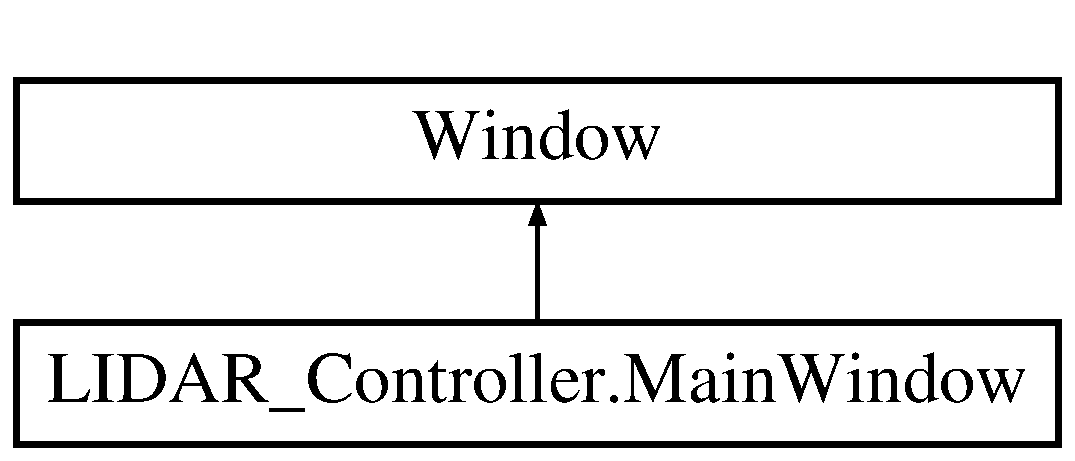
\includegraphics[height=2.000000cm]{class_l_i_d_a_r___controller_1_1_main_window}
\end{center}
\end{figure}
\subsection*{Public Member Functions}
\begin{DoxyCompactItemize}
\item 
\hyperlink{class_l_i_d_a_r___controller_1_1_main_window_adb6496654efc3e0d3d8b2db6b220252a}{Main\+Window} ()
\begin{DoxyCompactList}\small\item\em Default constructor of \hyperlink{class_l_i_d_a_r___controller_1_1_main_window}{Main\+Window}. This constructor does all the initialisation work. At first it initialises all G\+UI objects. Then it calls the init() function. This function adds C\+O\+M-\/\+Port informations to some G\+UI objects. The last function initializes the Viewport object. \end{DoxyCompactList}\end{DoxyCompactItemize}
\subsection*{Private Member Functions}
\begin{DoxyCompactItemize}
\item 
void \hyperlink{class_l_i_d_a_r___controller_1_1_main_window_a06e7e925f385b26d3fea4717bf359609}{Com\+Port\+Receive\+Handler} (object Sender, Serial\+Data\+Received\+Event\+Args e)
\begin{DoxyCompactList}\small\item\em Handler, called when the C\+O\+M-\/port receives something. \end{DoxyCompactList}\item 
void \hyperlink{class_l_i_d_a_r___controller_1_1_main_window_a1c0ad2dd56b20d3fdb928b918c0bc153}{Exeption\+Handler} (Exception ex) \textbackslash{}D+\char`\"{}
\begin{DoxyCompactList}\small\item\em Handler, called when a exception occurs. \end{DoxyCompactList}\item 
void \hyperlink{class_l_i_d_a_r___controller_1_1_main_window_a784f9cfcd0edd64ca5aa044112a34b49}{Init} ()
\begin{DoxyCompactList}\small\item\em Initialises both combo boxes with relevant data (e.\+g. available C\+O\+M-\/\+Ports). \end{DoxyCompactList}\item 
void \hyperlink{class_l_i_d_a_r___controller_1_1_main_window_a9d5c30796bf1dac53610783e94d10b37}{combo\+Box2\+\_\+\+Selection\+Changed} (object Sender, Selection\+Changed\+Event\+Args e)
\begin{DoxyCompactList}\small\item\em Event handler. Called by combo\+Box2 for selection changed events. This handler gets the offset values of the selected measurement and displays them. \end{DoxyCompactList}\item 
void \hyperlink{class_l_i_d_a_r___controller_1_1_main_window_acd58042bfc74176a4d65a7f7b9c8b455}{Init3D} ()
\begin{DoxyCompactList}\small\item\em Initialises the viewport object. \end{DoxyCompactList}\item 
void \hyperlink{class_l_i_d_a_r___controller_1_1_main_window_a2447b7c8a7d2310a89212d3cdc90e7f2}{verbinden\+\_\+\+Click} (object sender, Routed\+Event\+Args e)
\begin{DoxyCompactList}\small\item\em Event handler. Called by verbinden for click events. \end{DoxyCompactList}\item 
void \hyperlink{class_l_i_d_a_r___controller_1_1_main_window_a0be51e6fbf9c79cc4bbd40f41f044c47}{button2\+\_\+\+Click} (object sender, Routed\+Event\+Args e)
\begin{DoxyCompactList}\small\item\em Event handler. Called by button2 for click events. This functions sends the \char`\"{}\#1\char`\"{} (Onetime Measure) command to the L\+I\+D\+A\+R-\/\+Scanner. \end{DoxyCompactList}\item 
void \hyperlink{class_l_i_d_a_r___controller_1_1_main_window_a889652277fc1bd0a5f3e1aa584d30a20}{button3\+\_\+\+Click} (object sender, Routed\+Event\+Args e)
\begin{DoxyCompactList}\small\item\em Event handler. Called by button3 for click events. This functions sends the \char`\"{}\#2\char`\"{} (Radar mode 2D) command to the L\+I\+D\+A\+R-\/\+Scanner. \end{DoxyCompactList}\item 
void \hyperlink{class_l_i_d_a_r___controller_1_1_main_window_ac59530029320b9182c0db19ec2bb1344}{pos\+Btn\+\_\+\+Click} (object sender, Routed\+Event\+Args e)
\begin{DoxyCompactList}\small\item\em Event handler. Called by pos\+Btn for click events. This functions sends the \char`\"{}\#3\char`\"{} (Set Position) command with the position infos from \char`\"{}txt\+\_\+\+M\+Pos\char`\"{} \& \char`\"{}txt\+\_\+\+S\+Pos\char`\"{} to the L\+I\+D\+A\+R-\/\+Scanner. \end{DoxyCompactList}\item 
void \hyperlink{class_l_i_d_a_r___controller_1_1_main_window_a7819bd652f8bd6630e5879a7b101ec51}{button6\+\_\+\+Click} (object sender, Routed\+Event\+Args e)
\begin{DoxyCompactList}\small\item\em Event handler. Called by button6 for click events. This functions sends the \char`\"{}\#4\char`\"{} (Calibration) command to the L\+I\+D\+A\+R-\/\+Scanner. \end{DoxyCompactList}\item 
void \hyperlink{class_l_i_d_a_r___controller_1_1_main_window_ab831283d55f1beb21fcf043db6690c11}{neu\+Messung\+\_\+\+Click} (object sender, Routed\+Event\+Args e)
\begin{DoxyCompactList}\small\item\em Event handler. Called by neu\+Messung for click events. This function adds a new \hyperlink{class_l_i_d_a_r___controller_1_1_measurement}{Measurement} to Measure\+List and refreshes combobox2. \end{DoxyCompactList}\item 
void \hyperlink{class_l_i_d_a_r___controller_1_1_main_window_a94d838335feade09f122cad6a5600b74}{entf\+Messung\+\_\+\+Click} (object sender, Routed\+Event\+Args e)
\begin{DoxyCompactList}\small\item\em Event handler. Called by entf\+Messung for click events. This functions deletes the selected measurement and updates combobox2. \end{DoxyCompactList}\item 
void \hyperlink{class_l_i_d_a_r___controller_1_1_main_window_a786d1e5b609bbb158111051107ff860f}{offset\+Btn\+\_\+\+Click} (object sender, Routed\+Event\+Args e)
\begin{DoxyCompactList}\small\item\em Event handler. Called by offset\+Btn for click events. This function gets the offset information. Then id adds this values to the selected measurement. \end{DoxyCompactList}\item 
void \hyperlink{class_l_i_d_a_r___controller_1_1_main_window_a5897a8f1e59121209c0461bfd960b26a}{save\+Btn\+\_\+\+Click} (object sender, Routed\+Event\+Args e)
\begin{DoxyCompactList}\small\item\em Event handler. Called by save\+Btn for click events. Calls \char`\"{}\+D\+A\+O.\+save\+Measurements\char`\"{} to save all measurements to a xml file. \end{DoxyCompactList}\item 
void \hyperlink{class_l_i_d_a_r___controller_1_1_main_window_a3b7bbddaea2352a5c539b1d920a175b2}{load\+Btn\+\_\+\+Click} (object sender, Routed\+Event\+Args e)
\begin{DoxyCompactList}\small\item\em Event handler. Called by load\+Btn for click events. Calls \char`\"{}\+D\+A\+O.\+load\+Measurements\char`\"{} to load measurements from a xml file. \end{DoxyCompactList}\item 
void \hyperlink{class_l_i_d_a_r___controller_1_1_main_window_acea12fa391cab47bba07e6af85e4a765}{send\+Btn\+\_\+\+Click} (object sender, Routed\+Event\+Args e)
\begin{DoxyCompactList}\small\item\em Event handler. Called by send\+Btn for click events. This function sends the text of \char`\"{}send\+Txt\char`\"{} to the L\+I\+D\+A\+R-\/\+Scanner. \end{DoxyCompactList}\item 
void \hyperlink{class_l_i_d_a_r___controller_1_1_main_window_abc77995f990c7ef9dd53c0331b2c70a1}{enable\+Visuals} (bool b)
\begin{DoxyCompactList}\small\item\em Enables/\+Disables the visuals. \end{DoxyCompactList}\item 
void \hyperlink{class_l_i_d_a_r___controller_1_1_main_window_a644193ce9f107d5269d1443f8ff1d855}{reverse\+\_\+\+Click} (object sender, Routed\+Event\+Args e)
\begin{DoxyCompactList}\small\item\em Event handler. Called by reverse for click events. This function transforms the 3D model to a open/closed shape. \end{DoxyCompactList}\end{DoxyCompactItemize}
\subsection*{Private Attributes}
\begin{DoxyCompactItemize}
\item 
Serial\+Port \hyperlink{class_l_i_d_a_r___controller_1_1_main_window_ae8b01d789601ddbc234ede8a0b43eb7b}{Com\+Port} = null\hypertarget{class_l_i_d_a_r___controller_1_1_main_window_ae8b01d789601ddbc234ede8a0b43eb7b}{}\label{class_l_i_d_a_r___controller_1_1_main_window_ae8b01d789601ddbc234ede8a0b43eb7b}

\begin{DoxyCompactList}\small\item\em The C\+OM port which is used to communicate with the L\+I\+D\+A\+R-\/\+Scanner. \end{DoxyCompactList}\item 
int \hyperlink{class_l_i_d_a_r___controller_1_1_main_window_a01f677b33ad15d2f0cdf8df1c64cd0e2}{selected\+Measure}\hypertarget{class_l_i_d_a_r___controller_1_1_main_window_a01f677b33ad15d2f0cdf8df1c64cd0e2}{}\label{class_l_i_d_a_r___controller_1_1_main_window_a01f677b33ad15d2f0cdf8df1c64cd0e2}

\begin{DoxyCompactList}\small\item\em The actually selected measurement. \end{DoxyCompactList}\item 
List$<$ \hyperlink{class_l_i_d_a_r___controller_1_1_measurement}{Measurement} $>$ \hyperlink{class_l_i_d_a_r___controller_1_1_main_window_add7555b1a79fa1c17cd18dcf98859b9c}{Measure\+List} = new List$<$\hyperlink{class_l_i_d_a_r___controller_1_1_measurement}{Measurement}$>$()\hypertarget{class_l_i_d_a_r___controller_1_1_main_window_add7555b1a79fa1c17cd18dcf98859b9c}{}\label{class_l_i_d_a_r___controller_1_1_main_window_add7555b1a79fa1c17cd18dcf98859b9c}

\begin{DoxyCompactList}\small\item\em List of all measurements. \end{DoxyCompactList}\item 
Helix\+Viewport3D \hyperlink{class_l_i_d_a_r___controller_1_1_main_window_a4b0350fc0b7116a0d744ee8e489ab34a}{my\+Viewport} = new Helix\+Viewport3D()\hypertarget{class_l_i_d_a_r___controller_1_1_main_window_a4b0350fc0b7116a0d744ee8e489ab34a}{}\label{class_l_i_d_a_r___controller_1_1_main_window_a4b0350fc0b7116a0d744ee8e489ab34a}

\begin{DoxyCompactList}\small\item\em A viewport object that handles all 3\+D-\/\+Drawings. \end{DoxyCompactList}\item 
Grid\+Lines\+Visual3D \hyperlink{class_l_i_d_a_r___controller_1_1_main_window_a6be1b6eac4cf8176399dc7489e35f486}{grid\+Lines\+XY} = new Grid\+Lines\+Visual3D()\hypertarget{class_l_i_d_a_r___controller_1_1_main_window_a6be1b6eac4cf8176399dc7489e35f486}{}\label{class_l_i_d_a_r___controller_1_1_main_window_a6be1b6eac4cf8176399dc7489e35f486}

\begin{DoxyCompactList}\small\item\em The grid lines of the xy-\/plane. \end{DoxyCompactList}\end{DoxyCompactItemize}


\subsection{Detailed Description}
The application\textquotesingle{}s main form. This class contains all necessary event and exception handlers. 

\begin{DoxyAuthor}{Author}
Alexander Miller (7089316) 
\end{DoxyAuthor}
\begin{DoxyDate}{Date}
22.\+12.\+2015 
\end{DoxyDate}


Definition at line 31 of file Main\+Window.\+xaml.\+cs.



\subsection{Constructor \& Destructor Documentation}
\index{L\+I\+D\+A\+R\+\_\+\+Controller\+::\+Main\+Window@{L\+I\+D\+A\+R\+\_\+\+Controller\+::\+Main\+Window}!Main\+Window@{Main\+Window}}
\index{Main\+Window@{Main\+Window}!L\+I\+D\+A\+R\+\_\+\+Controller\+::\+Main\+Window@{L\+I\+D\+A\+R\+\_\+\+Controller\+::\+Main\+Window}}
\subsubsection[{\texorpdfstring{Main\+Window()}{MainWindow()}}]{\setlength{\rightskip}{0pt plus 5cm}public L\+I\+D\+A\+R\+\_\+\+Controller.\+Main\+Window.\+Main\+Window (
\begin{DoxyParamCaption}
{}
\end{DoxyParamCaption}
)}\hypertarget{class_l_i_d_a_r___controller_1_1_main_window_adb6496654efc3e0d3d8b2db6b220252a}{}\label{class_l_i_d_a_r___controller_1_1_main_window_adb6496654efc3e0d3d8b2db6b220252a}


Default constructor of \hyperlink{class_l_i_d_a_r___controller_1_1_main_window}{Main\+Window}. This constructor does all the initialisation work. At first it initialises all G\+UI objects. Then it calls the init() function. This function adds C\+O\+M-\/\+Port informations to some G\+UI objects. The last function initializes the Viewport object. 

\begin{DoxyAuthor}{Author}
Alexander Miller (7089316) 
\end{DoxyAuthor}
\begin{DoxyDate}{Date}
22.\+12.\+2015 
\end{DoxyDate}


Definition at line 65 of file Main\+Window.\+xaml.\+cs.


\begin{DoxyCode}
66         \{
67             InitializeComponent();
68             \hyperlink{class_l_i_d_a_r___controller_1_1_main_window_a784f9cfcd0edd64ca5aa044112a34b49}{Init}();
69             \hyperlink{class_l_i_d_a_r___controller_1_1_main_window_acd58042bfc74176a4d65a7f7b9c8b455}{Init3D}();
70         \}
\end{DoxyCode}


\subsection{Member Function Documentation}
\index{L\+I\+D\+A\+R\+\_\+\+Controller\+::\+Main\+Window@{L\+I\+D\+A\+R\+\_\+\+Controller\+::\+Main\+Window}!button2\+\_\+\+Click@{button2\+\_\+\+Click}}
\index{button2\+\_\+\+Click@{button2\+\_\+\+Click}!L\+I\+D\+A\+R\+\_\+\+Controller\+::\+Main\+Window@{L\+I\+D\+A\+R\+\_\+\+Controller\+::\+Main\+Window}}
\subsubsection[{\texorpdfstring{button2\+\_\+\+Click(object sender, Routed\+Event\+Args e)}{button2_Click(object sender, RoutedEventArgs e)}}]{\setlength{\rightskip}{0pt plus 5cm}private void L\+I\+D\+A\+R\+\_\+\+Controller.\+Main\+Window.\+button2\+\_\+\+Click (
\begin{DoxyParamCaption}
\item[{object}]{sender, }
\item[{Routed\+Event\+Args}]{e}
\end{DoxyParamCaption}
)\hspace{0.3cm}{\ttfamily [private]}}\hypertarget{class_l_i_d_a_r___controller_1_1_main_window_a0be51e6fbf9c79cc4bbd40f41f044c47}{}\label{class_l_i_d_a_r___controller_1_1_main_window_a0be51e6fbf9c79cc4bbd40f41f044c47}


Event handler. Called by button2 for click events. This functions sends the \char`\"{}\#1\char`\"{} (Onetime Measure) command to the L\+I\+D\+A\+R-\/\+Scanner. 

\begin{DoxyAuthor}{Author}
Alexander Miller (7089316) 
\end{DoxyAuthor}
\begin{DoxyDate}{Date}
22.\+12.\+2015
\end{DoxyDate}

\begin{DoxyParams}{Parameters}
{\em sender} & Source of the event. \\
\hline
{\em e} & Routed event information. \\
\hline
\end{DoxyParams}


Definition at line 361 of file Main\+Window.\+xaml.\+cs.


\begin{DoxyCode}
362         \{
363             \hyperlink{class_l_i_d_a_r___controller_1_1_main_window_ae8b01d789601ddbc234ede8a0b43eb7b}{ComPort}.WriteLine(\textcolor{stringliteral}{"#1"});
364         \}
\end{DoxyCode}
\index{L\+I\+D\+A\+R\+\_\+\+Controller\+::\+Main\+Window@{L\+I\+D\+A\+R\+\_\+\+Controller\+::\+Main\+Window}!button3\+\_\+\+Click@{button3\+\_\+\+Click}}
\index{button3\+\_\+\+Click@{button3\+\_\+\+Click}!L\+I\+D\+A\+R\+\_\+\+Controller\+::\+Main\+Window@{L\+I\+D\+A\+R\+\_\+\+Controller\+::\+Main\+Window}}
\subsubsection[{\texorpdfstring{button3\+\_\+\+Click(object sender, Routed\+Event\+Args e)}{button3_Click(object sender, RoutedEventArgs e)}}]{\setlength{\rightskip}{0pt plus 5cm}private void L\+I\+D\+A\+R\+\_\+\+Controller.\+Main\+Window.\+button3\+\_\+\+Click (
\begin{DoxyParamCaption}
\item[{object}]{sender, }
\item[{Routed\+Event\+Args}]{e}
\end{DoxyParamCaption}
)\hspace{0.3cm}{\ttfamily [private]}}\hypertarget{class_l_i_d_a_r___controller_1_1_main_window_a889652277fc1bd0a5f3e1aa584d30a20}{}\label{class_l_i_d_a_r___controller_1_1_main_window_a889652277fc1bd0a5f3e1aa584d30a20}


Event handler. Called by button3 for click events. This functions sends the \char`\"{}\#2\char`\"{} (Radar mode 2D) command to the L\+I\+D\+A\+R-\/\+Scanner. 

\begin{DoxyAuthor}{Author}
Alexander Miller (7089316) 
\end{DoxyAuthor}
\begin{DoxyDate}{Date}
22.\+12.\+2015
\end{DoxyDate}

\begin{DoxyParams}{Parameters}
{\em sender} & Source of the event. \\
\hline
{\em e} & Routed event information. \\
\hline
\end{DoxyParams}


Definition at line 379 of file Main\+Window.\+xaml.\+cs.


\begin{DoxyCode}
380         \{
381             \hyperlink{class_l_i_d_a_r___controller_1_1_main_window_ae8b01d789601ddbc234ede8a0b43eb7b}{ComPort}.WriteLine(\textcolor{stringliteral}{"#2"});
382         \}
\end{DoxyCode}
\index{L\+I\+D\+A\+R\+\_\+\+Controller\+::\+Main\+Window@{L\+I\+D\+A\+R\+\_\+\+Controller\+::\+Main\+Window}!button6\+\_\+\+Click@{button6\+\_\+\+Click}}
\index{button6\+\_\+\+Click@{button6\+\_\+\+Click}!L\+I\+D\+A\+R\+\_\+\+Controller\+::\+Main\+Window@{L\+I\+D\+A\+R\+\_\+\+Controller\+::\+Main\+Window}}
\subsubsection[{\texorpdfstring{button6\+\_\+\+Click(object sender, Routed\+Event\+Args e)}{button6_Click(object sender, RoutedEventArgs e)}}]{\setlength{\rightskip}{0pt plus 5cm}private void L\+I\+D\+A\+R\+\_\+\+Controller.\+Main\+Window.\+button6\+\_\+\+Click (
\begin{DoxyParamCaption}
\item[{object}]{sender, }
\item[{Routed\+Event\+Args}]{e}
\end{DoxyParamCaption}
)\hspace{0.3cm}{\ttfamily [private]}}\hypertarget{class_l_i_d_a_r___controller_1_1_main_window_a7819bd652f8bd6630e5879a7b101ec51}{}\label{class_l_i_d_a_r___controller_1_1_main_window_a7819bd652f8bd6630e5879a7b101ec51}


Event handler. Called by button6 for click events. This functions sends the \char`\"{}\#4\char`\"{} (Calibration) command to the L\+I\+D\+A\+R-\/\+Scanner. 

\begin{DoxyAuthor}{Author}
Alexander Miller (7089316) 
\end{DoxyAuthor}
\begin{DoxyDate}{Date}
22.\+12.\+2015
\end{DoxyDate}

\begin{DoxyParams}{Parameters}
{\em sender} & Source of the event. \\
\hline
{\em e} & Routed event information. \\
\hline
\end{DoxyParams}


Definition at line 427 of file Main\+Window.\+xaml.\+cs.


\begin{DoxyCode}
428         \{
429             \hyperlink{class_l_i_d_a_r___controller_1_1_main_window_ae8b01d789601ddbc234ede8a0b43eb7b}{ComPort}.WriteLine(\textcolor{stringliteral}{"#4"});
430         \}
\end{DoxyCode}
\index{L\+I\+D\+A\+R\+\_\+\+Controller\+::\+Main\+Window@{L\+I\+D\+A\+R\+\_\+\+Controller\+::\+Main\+Window}!combo\+Box2\+\_\+\+Selection\+Changed@{combo\+Box2\+\_\+\+Selection\+Changed}}
\index{combo\+Box2\+\_\+\+Selection\+Changed@{combo\+Box2\+\_\+\+Selection\+Changed}!L\+I\+D\+A\+R\+\_\+\+Controller\+::\+Main\+Window@{L\+I\+D\+A\+R\+\_\+\+Controller\+::\+Main\+Window}}
\subsubsection[{\texorpdfstring{combo\+Box2\+\_\+\+Selection\+Changed(object Sender, Selection\+Changed\+Event\+Args e)}{comboBox2_SelectionChanged(object Sender, SelectionChangedEventArgs e)}}]{\setlength{\rightskip}{0pt plus 5cm}void L\+I\+D\+A\+R\+\_\+\+Controller.\+Main\+Window.\+combo\+Box2\+\_\+\+Selection\+Changed (
\begin{DoxyParamCaption}
\item[{object}]{Sender, }
\item[{Selection\+Changed\+Event\+Args}]{e}
\end{DoxyParamCaption}
)\hspace{0.3cm}{\ttfamily [private]}}\hypertarget{class_l_i_d_a_r___controller_1_1_main_window_a9d5c30796bf1dac53610783e94d10b37}{}\label{class_l_i_d_a_r___controller_1_1_main_window_a9d5c30796bf1dac53610783e94d10b37}


Event handler. Called by combo\+Box2 for selection changed events. This handler gets the offset values of the selected measurement and displays them. 

\begin{DoxyAuthor}{Author}
Alexander Miller (7089316) 
\end{DoxyAuthor}
\begin{DoxyDate}{Date}
22.\+12.\+2015
\end{DoxyDate}

\begin{DoxyParams}{Parameters}
{\em Sender} & Source of the event. \\
\hline
{\em e} & Selection changed event information. \\
\hline
\end{DoxyParams}


Definition at line 206 of file Main\+Window.\+xaml.\+cs.


\begin{DoxyCode}
207         \{
208             \hyperlink{class_l_i_d_a_r___controller_1_1_main_window_a01f677b33ad15d2f0cdf8df1c64cd0e2}{selectedMeasure} = comboBox2.SelectedIndex;
209             \textcolor{keywordflow}{if} (\hyperlink{class_l_i_d_a_r___controller_1_1_main_window_a01f677b33ad15d2f0cdf8df1c64cd0e2}{selectedMeasure} >= 0)
210             \{
211                 xOffsetTxt.Text = \textcolor{stringliteral}{""} + \hyperlink{class_l_i_d_a_r___controller_1_1_main_window_add7555b1a79fa1c17cd18dcf98859b9c}{MeasureList}[\hyperlink{class_l_i_d_a_r___controller_1_1_main_window_a01f677b33ad15d2f0cdf8df1c64cd0e2}{selectedMeasure}].linearOffset.
      X;
212                 yOffsetTxt.Text = \textcolor{stringliteral}{""} + \hyperlink{class_l_i_d_a_r___controller_1_1_main_window_add7555b1a79fa1c17cd18dcf98859b9c}{MeasureList}[\hyperlink{class_l_i_d_a_r___controller_1_1_main_window_a01f677b33ad15d2f0cdf8df1c64cd0e2}{selectedMeasure}].linearOffset.
      Y;
213                 zOffsetTxt.Text = \textcolor{stringliteral}{""} + \hyperlink{class_l_i_d_a_r___controller_1_1_main_window_add7555b1a79fa1c17cd18dcf98859b9c}{MeasureList}[\hyperlink{class_l_i_d_a_r___controller_1_1_main_window_a01f677b33ad15d2f0cdf8df1c64cd0e2}{selectedMeasure}].linearOffset.
      Z;
214                 degOffsetXTxt.Text = \textcolor{stringliteral}{""} + \hyperlink{class_l_i_d_a_r___controller_1_1_main_window_add7555b1a79fa1c17cd18dcf98859b9c}{MeasureList}[\hyperlink{class_l_i_d_a_r___controller_1_1_main_window_a01f677b33ad15d2f0cdf8df1c64cd0e2}{selectedMeasure}].
      rotaryOffsetX;
215                 degOffsetZTxt.Text = \textcolor{stringliteral}{""} + \hyperlink{class_l_i_d_a_r___controller_1_1_main_window_add7555b1a79fa1c17cd18dcf98859b9c}{MeasureList}[\hyperlink{class_l_i_d_a_r___controller_1_1_main_window_a01f677b33ad15d2f0cdf8df1c64cd0e2}{selectedMeasure}].
      rotaryOffsetZ;
216             \}
217 
218         \}
\end{DoxyCode}
\index{L\+I\+D\+A\+R\+\_\+\+Controller\+::\+Main\+Window@{L\+I\+D\+A\+R\+\_\+\+Controller\+::\+Main\+Window}!Com\+Port\+Receive\+Handler@{Com\+Port\+Receive\+Handler}}
\index{Com\+Port\+Receive\+Handler@{Com\+Port\+Receive\+Handler}!L\+I\+D\+A\+R\+\_\+\+Controller\+::\+Main\+Window@{L\+I\+D\+A\+R\+\_\+\+Controller\+::\+Main\+Window}}
\subsubsection[{\texorpdfstring{Com\+Port\+Receive\+Handler(object Sender, Serial\+Data\+Received\+Event\+Args e)}{ComPortReceiveHandler(object Sender, SerialDataReceivedEventArgs e)}}]{\setlength{\rightskip}{0pt plus 5cm}private void L\+I\+D\+A\+R\+\_\+\+Controller.\+Main\+Window.\+Com\+Port\+Receive\+Handler (
\begin{DoxyParamCaption}
\item[{object}]{Sender, }
\item[{Serial\+Data\+Received\+Event\+Args}]{e}
\end{DoxyParamCaption}
)\hspace{0.3cm}{\ttfamily [private]}}\hypertarget{class_l_i_d_a_r___controller_1_1_main_window_a06e7e925f385b26d3fea4717bf359609}{}\label{class_l_i_d_a_r___controller_1_1_main_window_a06e7e925f385b26d3fea4717bf359609}


Handler, called when the C\+O\+M-\/port receives something. 

a\+: if no problems occur then...


\begin{DoxyEnumerate}
\item Check if Com\+Port is open
\item Read line from buffer
\item Add the received line to text\+Box1
\item Get relevant data from string using a regular expression
\item Parse data into integers
\item Set a point of the selected measurement based on the received data.
\end{DoxyEnumerate}

b\+: If something goes wrong, call the exception handler.

\begin{DoxyAuthor}{Author}
Alexander Miller (7089316) 
\end{DoxyAuthor}
\begin{DoxyDate}{Date}
22.\+12.\+2015
\end{DoxyDate}

\begin{DoxyParams}{Parameters}
{\em Sender} & Source of the event. \\
\hline
{\em e} & Serial data received event information. \\
\hline
\end{DoxyParams}


Definition at line 95 of file Main\+Window.\+xaml.\+cs.


\begin{DoxyCode}
96         \{
97             \textcolor{comment}{//a}
98             \textcolor{keywordflow}{try}
99             \{
100                 \textcolor{comment}{//1}
101                 \textcolor{keywordflow}{if} (!\hyperlink{class_l_i_d_a_r___controller_1_1_main_window_ae8b01d789601ddbc234ede8a0b43eb7b}{ComPort}.IsOpen) \textcolor{keywordflow}{return};
102                 \textcolor{keywordtype}{string} ReceivedText = \textcolor{stringliteral}{""};
103                 \textcolor{comment}{//2}
104                 ReceivedText = \hyperlink{class_l_i_d_a_r___controller_1_1_main_window_ae8b01d789601ddbc234ede8a0b43eb7b}{ComPort}.ReadLine();
105                 \textcolor{comment}{//3}
106                 Dispatcher.BeginInvoke(\textcolor{keyword}{new} Action(() =>
107                 \{
108                     this.textBox1.AppendText(ReceivedText);
109                     this.textBox1.ScrollToEnd();
110                 \}));
111                 \textcolor{comment}{//4}
112                 \textcolor{keywordtype}{string}[] numbers = Regex.Split(ReceivedText, \textcolor{stringliteral}{@"\(\backslash\)D+"});
113                 \textcolor{comment}{//5}
114                 \textcolor{keywordflow}{if} (numbers.Length == 5)
115                 \{
116                     \textcolor{keywordtype}{int} mpos = 0;
117                     \textcolor{keywordtype}{int} spos = 0;
118                     \textcolor{keywordtype}{int} value = 0;
119                     \textcolor{keywordflow}{if} (\textcolor{keywordtype}{int}.TryParse(numbers[1], out mpos) && \textcolor{keywordtype}{int}.TryParse(numbers[2], out spos) && \textcolor{keywordtype}{int}.
      TryParse(numbers[3],out value))
120                         \textcolor{comment}{//6}
121                         \hyperlink{class_l_i_d_a_r___controller_1_1_main_window_add7555b1a79fa1c17cd18dcf98859b9c}{MeasureList}[\hyperlink{class_l_i_d_a_r___controller_1_1_main_window_a01f677b33ad15d2f0cdf8df1c64cd0e2}{selectedMeasure}].setDistanceData(mpos+1, spos
      , value);
122                     Dispatcher.BeginInvoke(\textcolor{keyword}{new} Action(() =>
123                     \{
124                         \hyperlink{class_l_i_d_a_r___controller_1_1_main_window_add7555b1a79fa1c17cd18dcf98859b9c}{MeasureList}[\hyperlink{class_l_i_d_a_r___controller_1_1_main_window_a01f677b33ad15d2f0cdf8df1c64cd0e2}{selectedMeasure}].setGeometryPoint3D(mpos+1 , 
      spos);
125 
126                     \}));
127 
128 
129 
130                 \}
131             \}
132             \textcolor{comment}{//b}
133             \textcolor{keywordflow}{catch} (Exception ex) \{ \hyperlink{class_l_i_d_a_r___controller_1_1_main_window_a1c0ad2dd56b20d3fdb928b918c0bc153}{ExeptionHandler}(ex); \}
134         \}
\end{DoxyCode}
\index{L\+I\+D\+A\+R\+\_\+\+Controller\+::\+Main\+Window@{L\+I\+D\+A\+R\+\_\+\+Controller\+::\+Main\+Window}!enable\+Visuals@{enable\+Visuals}}
\index{enable\+Visuals@{enable\+Visuals}!L\+I\+D\+A\+R\+\_\+\+Controller\+::\+Main\+Window@{L\+I\+D\+A\+R\+\_\+\+Controller\+::\+Main\+Window}}
\subsubsection[{\texorpdfstring{enable\+Visuals(bool b)}{enableVisuals(bool b)}}]{\setlength{\rightskip}{0pt plus 5cm}private void L\+I\+D\+A\+R\+\_\+\+Controller.\+Main\+Window.\+enable\+Visuals (
\begin{DoxyParamCaption}
\item[{bool}]{b}
\end{DoxyParamCaption}
)\hspace{0.3cm}{\ttfamily [private]}}\hypertarget{class_l_i_d_a_r___controller_1_1_main_window_abc77995f990c7ef9dd53c0331b2c70a1}{}\label{class_l_i_d_a_r___controller_1_1_main_window_abc77995f990c7ef9dd53c0331b2c70a1}


Enables/\+Disables the visuals. 

\begin{DoxyAuthor}{Author}
Alexander Miller (7089316) 
\end{DoxyAuthor}
\begin{DoxyDate}{Date}
22.\+12.\+2015
\end{DoxyDate}

\begin{DoxyParams}{Parameters}
{\em b} & true enables visuals and false disables them. \\
\hline
\end{DoxyParams}


Definition at line 654 of file Main\+Window.\+xaml.\+cs.


\begin{DoxyCode}
655         \{
656             \textcolor{comment}{//neuMessung.IsEnabled = b;}
657             \textcolor{comment}{//entfMessung.IsEnabled = b;}
658             \textcolor{comment}{//offsetBtn.IsEnabled = b;}
659             btn\_einzelmessung.IsEnabled = b;
660             btn\_kalibrieren.IsEnabled = b;
661             posBtn.IsEnabled = b;
662             btn\_radar.IsEnabled = b;
663             txt\_MPos.IsEnabled = b;
664             txt\_SPos.IsEnabled = b;
665             \textcolor{comment}{//sendBtn.IsEnabled = b;}
666             \textcolor{comment}{//comboBox2.IsEnabled = b;}
667             \textcolor{comment}{//sendTxt.IsEnabled = b;}
668             \textcolor{comment}{//txt\_punktmessung.IsEnabled = b;}
669             \textcolor{comment}{//xOffsetTxt.IsEnabled = b;}
670             \textcolor{comment}{//yOffsetTxt.IsEnabled = b;}
671             \textcolor{comment}{//zOffsetTxt.IsEnabled = b;}
672             \textcolor{comment}{//degOffsetTxt.IsEnabled = b;}
673             \textcolor{comment}{//textBox1.IsEnabled = b;}
674         \}
\end{DoxyCode}
\index{L\+I\+D\+A\+R\+\_\+\+Controller\+::\+Main\+Window@{L\+I\+D\+A\+R\+\_\+\+Controller\+::\+Main\+Window}!entf\+Messung\+\_\+\+Click@{entf\+Messung\+\_\+\+Click}}
\index{entf\+Messung\+\_\+\+Click@{entf\+Messung\+\_\+\+Click}!L\+I\+D\+A\+R\+\_\+\+Controller\+::\+Main\+Window@{L\+I\+D\+A\+R\+\_\+\+Controller\+::\+Main\+Window}}
\subsubsection[{\texorpdfstring{entf\+Messung\+\_\+\+Click(object sender, Routed\+Event\+Args e)}{entfMessung_Click(object sender, RoutedEventArgs e)}}]{\setlength{\rightskip}{0pt plus 5cm}private void L\+I\+D\+A\+R\+\_\+\+Controller.\+Main\+Window.\+entf\+Messung\+\_\+\+Click (
\begin{DoxyParamCaption}
\item[{object}]{sender, }
\item[{Routed\+Event\+Args}]{e}
\end{DoxyParamCaption}
)\hspace{0.3cm}{\ttfamily [private]}}\hypertarget{class_l_i_d_a_r___controller_1_1_main_window_a94d838335feade09f122cad6a5600b74}{}\label{class_l_i_d_a_r___controller_1_1_main_window_a94d838335feade09f122cad6a5600b74}


Event handler. Called by entf\+Messung for click events. This functions deletes the selected measurement and updates combobox2. 


\begin{DoxyEnumerate}
\item Check if at least 2 measurements are available
\item Remove the selected measurement form Measure\+List
\item Clear combobox2
\item Add all remaining measurements to combobox2
\item Reset my\+Viewport
\item Add all remaining measurements to my\+Viewport as children to display them
\end{DoxyEnumerate}

\begin{DoxyAuthor}{Author}
Alexander Miller (7089316) 
\end{DoxyAuthor}
\begin{DoxyDate}{Date}
22.\+12.\+2015
\end{DoxyDate}

\begin{DoxyParams}{Parameters}
{\em sender} & Source of the event. \\
\hline
{\em e} & Routed event information. \\
\hline
\end{DoxyParams}


Definition at line 486 of file Main\+Window.\+xaml.\+cs.


\begin{DoxyCode}
487         \{
488             \textcolor{comment}{//1}
489             \textcolor{keywordflow}{if} (\hyperlink{class_l_i_d_a_r___controller_1_1_main_window_add7555b1a79fa1c17cd18dcf98859b9c}{MeasureList}.Count > 1)
490             \{
491                 \textcolor{comment}{//2}
492                 \hyperlink{class_l_i_d_a_r___controller_1_1_main_window_add7555b1a79fa1c17cd18dcf98859b9c}{MeasureList}.RemoveAt(\hyperlink{class_l_i_d_a_r___controller_1_1_main_window_a01f677b33ad15d2f0cdf8df1c64cd0e2}{selectedMeasure});
493                 \textcolor{comment}{//3}
494                 comboBox2.Items.Clear();
495                 \textcolor{comment}{//4}
496                 \textcolor{keywordflow}{foreach} (Measurement x \textcolor{keywordflow}{in} \hyperlink{class_l_i_d_a_r___controller_1_1_main_window_add7555b1a79fa1c17cd18dcf98859b9c}{MeasureList})
497                 \{
498                     comboBox2.Items.Add(x);
499                 \}
500                 comboBox2.SelectedIndex = 0;
501                 \textcolor{comment}{//5}
502                 \hyperlink{class_l_i_d_a_r___controller_1_1_main_window_a4b0350fc0b7116a0d744ee8e489ab34a}{myViewport}.Children.Clear();
503                 \textcolor{comment}{//6}
504                 \hyperlink{class_l_i_d_a_r___controller_1_1_main_window_a4b0350fc0b7116a0d744ee8e489ab34a}{myViewport}.Children.Add(\hyperlink{class_l_i_d_a_r___controller_1_1_main_window_a6be1b6eac4cf8176399dc7489e35f486}{gridLinesXY});
505                 \hyperlink{class_l_i_d_a_r___controller_1_1_main_window_a4b0350fc0b7116a0d744ee8e489ab34a}{myViewport}.Children.Add(\textcolor{keyword}{new} DefaultLights());
506                 \textcolor{keywordflow}{foreach} (Measurement x \textcolor{keywordflow}{in} MeasureList)
507                 \{
508                     \hyperlink{class_l_i_d_a_r___controller_1_1_main_window_a4b0350fc0b7116a0d744ee8e489ab34a}{myViewport}.Children.Add(x.getGeometry3D());
509                 \}
510             \}
511 
512 
513         \}
\end{DoxyCode}
\index{L\+I\+D\+A\+R\+\_\+\+Controller\+::\+Main\+Window@{L\+I\+D\+A\+R\+\_\+\+Controller\+::\+Main\+Window}!Exeption\+Handler@{Exeption\+Handler}}
\index{Exeption\+Handler@{Exeption\+Handler}!L\+I\+D\+A\+R\+\_\+\+Controller\+::\+Main\+Window@{L\+I\+D\+A\+R\+\_\+\+Controller\+::\+Main\+Window}}
\subsubsection[{\texorpdfstring{Exeption\+Handler(\+Exception ex)}{ExeptionHandler(Exception ex)}}]{\setlength{\rightskip}{0pt plus 5cm}private void L\+I\+D\+A\+R\+\_\+\+Controller.\+Main\+Window.\+Exeption\+Handler (
\begin{DoxyParamCaption}
\item[{Exception}]{ex}
\end{DoxyParamCaption}
) \textbackslash{}D+\char`\"{}\hspace{0.3cm}{\ttfamily [private]}}\hypertarget{class_l_i_d_a_r___controller_1_1_main_window_a1c0ad2dd56b20d3fdb928b918c0bc153}{}\label{class_l_i_d_a_r___controller_1_1_main_window_a1c0ad2dd56b20d3fdb928b918c0bc153}


Handler, called when a exception occurs. 

\begin{DoxyAuthor}{Author}
Alexander Miller (7089316) 
\end{DoxyAuthor}
\begin{DoxyDate}{Date}
22.\+12.\+2015
\end{DoxyDate}

\begin{DoxyParams}{Parameters}
{\em ex} & The exception that occurred. \\
\hline
\end{DoxyParams}


Definition at line 147 of file Main\+Window.\+xaml.\+cs.


\begin{DoxyCode}
148         \{
149             \textcolor{keywordflow}{switch} (ex.GetType().Name)
150             \{
151                 \textcolor{keywordflow}{case} \textcolor{stringliteral}{"IOException"}:
152                     MessageBox.Show(\textcolor{stringliteral}{"Name: "} + ex.GetType().Name + \textcolor{stringliteral}{"\(\backslash\)r\(\backslash\)nBeschreibung:\(\backslash\)r\(\backslash\)n"} + ex.Message, \textcolor{stringliteral}{"
      Fehler!"}, MessageBoxButton.OK, MessageBoxImage.Error);
153                     \textcolor{keywordflow}{break};
154                 \textcolor{keywordflow}{case} \textcolor{stringliteral}{"ArgumentException"}:
155                     MessageBox.Show(\textcolor{stringliteral}{"Bitte Eingaben überprüfen!"}, \textcolor{stringliteral}{"Fehleingabe erkannt!"}, MessageBoxButton.
      OK, MessageBoxImage.Information);
156                     \textcolor{keywordflow}{break};
157                 \textcolor{keywordflow}{default}:
158                     MessageBox.Show(\textcolor{stringliteral}{"Name: "} + ex.GetType().Name + \textcolor{stringliteral}{"\(\backslash\)r\(\backslash\)nBeschreibung:\(\backslash\)r\(\backslash\)n"} + ex.Message, \textcolor{stringliteral}{"
      Unbekannter Fehler!"}, MessageBoxButton.OK, MessageBoxImage.Error);
159                     \textcolor{keywordflow}{break};
160             \}
161 
162         \}
\end{DoxyCode}
\index{L\+I\+D\+A\+R\+\_\+\+Controller\+::\+Main\+Window@{L\+I\+D\+A\+R\+\_\+\+Controller\+::\+Main\+Window}!Init@{Init}}
\index{Init@{Init}!L\+I\+D\+A\+R\+\_\+\+Controller\+::\+Main\+Window@{L\+I\+D\+A\+R\+\_\+\+Controller\+::\+Main\+Window}}
\subsubsection[{\texorpdfstring{Init()}{Init()}}]{\setlength{\rightskip}{0pt plus 5cm}private void L\+I\+D\+A\+R\+\_\+\+Controller.\+Main\+Window.\+Init (
\begin{DoxyParamCaption}
{}
\end{DoxyParamCaption}
)\hspace{0.3cm}{\ttfamily [private]}}\hypertarget{class_l_i_d_a_r___controller_1_1_main_window_a784f9cfcd0edd64ca5aa044112a34b49}{}\label{class_l_i_d_a_r___controller_1_1_main_window_a784f9cfcd0edd64ca5aa044112a34b49}


Initialises both combo boxes with relevant data (e.\+g. available C\+O\+M-\/\+Ports). 

\begin{DoxyAuthor}{Author}
Alexander Miller (7089316) 
\end{DoxyAuthor}
\begin{DoxyDate}{Date}
22.\+12.\+2015 
\end{DoxyDate}


Definition at line 173 of file Main\+Window.\+xaml.\+cs.


\begin{DoxyCode}
174         \{
175             \textcolor{comment}{//add all COM-Ports to combobox}
176             \textcolor{keywordflow}{foreach} (\textcolor{keywordtype}{string} ports \textcolor{keywordflow}{in} SerialPort.GetPortNames())
177             \{
178                 comboBox.Items.Add(ports);
179             \}
180             \textcolor{comment}{//initial measurement}
181             \hyperlink{class_l_i_d_a_r___controller_1_1_main_window_add7555b1a79fa1c17cd18dcf98859b9c}{MeasureList}.Add(\textcolor{keyword}{new} Measurement(\textcolor{keyword}{new} Vector3D(0, 0, 0.5), 0, 0));
182 
183             \textcolor{comment}{//add measurement to combobox2 and register a new event handler for "SelectionChangedEvent"}
184             comboBox2.Items.Add(\hyperlink{class_l_i_d_a_r___controller_1_1_main_window_add7555b1a79fa1c17cd18dcf98859b9c}{MeasureList}[\hyperlink{class_l_i_d_a_r___controller_1_1_main_window_a01f677b33ad15d2f0cdf8df1c64cd0e2}{selectedMeasure}]);
185             comboBox2.DisplayMemberPath = \textcolor{stringliteral}{"mId"};
186             comboBox2.SelectionChanged += \textcolor{keyword}{new} SelectionChangedEventHandler(
      \hyperlink{class_l_i_d_a_r___controller_1_1_main_window_a9d5c30796bf1dac53610783e94d10b37}{comboBox2\_SelectionChanged});
187             comboBox2.SelectedIndex = 0;
188             \textcolor{comment}{//Enable/Disable all GUI-Elements that need a connected COM-Port}
189             \hyperlink{class_l_i_d_a_r___controller_1_1_main_window_abc77995f990c7ef9dd53c0331b2c70a1}{enableVisuals}(\textcolor{keyword}{false});
190 
191         \}
\end{DoxyCode}
\index{L\+I\+D\+A\+R\+\_\+\+Controller\+::\+Main\+Window@{L\+I\+D\+A\+R\+\_\+\+Controller\+::\+Main\+Window}!Init3D@{Init3D}}
\index{Init3D@{Init3D}!L\+I\+D\+A\+R\+\_\+\+Controller\+::\+Main\+Window@{L\+I\+D\+A\+R\+\_\+\+Controller\+::\+Main\+Window}}
\subsubsection[{\texorpdfstring{Init3\+D()}{Init3D()}}]{\setlength{\rightskip}{0pt plus 5cm}private void L\+I\+D\+A\+R\+\_\+\+Controller.\+Main\+Window.\+Init3D (
\begin{DoxyParamCaption}
{}
\end{DoxyParamCaption}
)\hspace{0.3cm}{\ttfamily [private]}}\hypertarget{class_l_i_d_a_r___controller_1_1_main_window_acd58042bfc74176a4d65a7f7b9c8b455}{}\label{class_l_i_d_a_r___controller_1_1_main_window_acd58042bfc74176a4d65a7f7b9c8b455}


Initialises the viewport object. 


\begin{DoxyEnumerate}
\item Configure the grid lines for the xy-\/\+Plane.
\item Configure my\+Viewport to show additional data.
\item Add grid\+Lines\+XY, a default light and the 3\+D-\/\+Model of the selected measurement to my\+Viewport as children.
\item Add my\+Viewport to grid (G\+U\+I-\/\+Element) as child and refresh.
\end{DoxyEnumerate}

\begin{DoxyAuthor}{Author}
Alexander Miller (7089316) 
\end{DoxyAuthor}
\begin{DoxyDate}{Date}
22.\+12.\+2015 
\end{DoxyDate}


Definition at line 233 of file Main\+Window.\+xaml.\+cs.


\begin{DoxyCode}
234         \{
235             \textcolor{comment}{//1}
236             \hyperlink{class_l_i_d_a_r___controller_1_1_main_window_a6be1b6eac4cf8176399dc7489e35f486}{gridLinesXY}.MinorDistance = 10; \textcolor{comment}{//Distance in cm for the minor lines }
237             \hyperlink{class_l_i_d_a_r___controller_1_1_main_window_a6be1b6eac4cf8176399dc7489e35f486}{gridLinesXY}.MajorDistance = 100; \textcolor{comment}{//Distance in cm for the major lines }
238             \hyperlink{class_l_i_d_a_r___controller_1_1_main_window_a6be1b6eac4cf8176399dc7489e35f486}{gridLinesXY}.Thickness = 1.5; \textcolor{comment}{//Line thickness}
239             \hyperlink{class_l_i_d_a_r___controller_1_1_main_window_a6be1b6eac4cf8176399dc7489e35f486}{gridLinesXY}.Length = 10000; \textcolor{comment}{//Maximum grid size}
240             \hyperlink{class_l_i_d_a_r___controller_1_1_main_window_a6be1b6eac4cf8176399dc7489e35f486}{gridLinesXY}.Width = 10000; \textcolor{comment}{//Maximum grid size}
241 
242             \textcolor{comment}{//2}
243             \hyperlink{class_l_i_d_a_r___controller_1_1_main_window_a4b0350fc0b7116a0d744ee8e489ab34a}{myViewport}.ShowFrameRate = \textcolor{keyword}{true}; \textcolor{comment}{//Show framerate}
244             \hyperlink{class_l_i_d_a_r___controller_1_1_main_window_a4b0350fc0b7116a0d744ee8e489ab34a}{myViewport}.ShowCoordinateSystem = \textcolor{keyword}{true}; \textcolor{comment}{//Show small Coordinate system}
245             \hyperlink{class_l_i_d_a_r___controller_1_1_main_window_a4b0350fc0b7116a0d744ee8e489ab34a}{myViewport}.ShowFieldOfView = \textcolor{keyword}{true}; \textcolor{comment}{//Show Field of View}
246 
247             \textcolor{comment}{//3}
248             \hyperlink{class_l_i_d_a_r___controller_1_1_main_window_a4b0350fc0b7116a0d744ee8e489ab34a}{myViewport}.Children.Add(\hyperlink{class_l_i_d_a_r___controller_1_1_main_window_a6be1b6eac4cf8176399dc7489e35f486}{gridLinesXY});
249             \hyperlink{class_l_i_d_a_r___controller_1_1_main_window_a4b0350fc0b7116a0d744ee8e489ab34a}{myViewport}.Children.Add(\textcolor{keyword}{new} DefaultLights());
250             \hyperlink{class_l_i_d_a_r___controller_1_1_main_window_a4b0350fc0b7116a0d744ee8e489ab34a}{myViewport}.Children.Add(\hyperlink{class_l_i_d_a_r___controller_1_1_main_window_add7555b1a79fa1c17cd18dcf98859b9c}{MeasureList}[
      \hyperlink{class_l_i_d_a_r___controller_1_1_main_window_a01f677b33ad15d2f0cdf8df1c64cd0e2}{selectedMeasure}].getGeometry3D());
251 
252             \textcolor{comment}{//4}
253             grid.Children.Add(\hyperlink{class_l_i_d_a_r___controller_1_1_main_window_a4b0350fc0b7116a0d744ee8e489ab34a}{myViewport});
254             grid.UpdateLayout();
255 
256         \}
\end{DoxyCode}
\index{L\+I\+D\+A\+R\+\_\+\+Controller\+::\+Main\+Window@{L\+I\+D\+A\+R\+\_\+\+Controller\+::\+Main\+Window}!load\+Btn\+\_\+\+Click@{load\+Btn\+\_\+\+Click}}
\index{load\+Btn\+\_\+\+Click@{load\+Btn\+\_\+\+Click}!L\+I\+D\+A\+R\+\_\+\+Controller\+::\+Main\+Window@{L\+I\+D\+A\+R\+\_\+\+Controller\+::\+Main\+Window}}
\subsubsection[{\texorpdfstring{load\+Btn\+\_\+\+Click(object sender, Routed\+Event\+Args e)}{loadBtn_Click(object sender, RoutedEventArgs e)}}]{\setlength{\rightskip}{0pt plus 5cm}private void L\+I\+D\+A\+R\+\_\+\+Controller.\+Main\+Window.\+load\+Btn\+\_\+\+Click (
\begin{DoxyParamCaption}
\item[{object}]{sender, }
\item[{Routed\+Event\+Args}]{e}
\end{DoxyParamCaption}
)\hspace{0.3cm}{\ttfamily [private]}}\hypertarget{class_l_i_d_a_r___controller_1_1_main_window_a3b7bbddaea2352a5c539b1d920a175b2}{}\label{class_l_i_d_a_r___controller_1_1_main_window_a3b7bbddaea2352a5c539b1d920a175b2}


Event handler. Called by load\+Btn for click events. Calls \char`\"{}\+D\+A\+O.\+load\+Measurements\char`\"{} to load measurements from a xml file. 


\begin{DoxyEnumerate}
\item Get a list of Measurements from a xml file
\item Clear combobox2
\item Add all measurements to combobox2
\item Reset my\+Viewport
\item Add all measurements to my\+Viewport as children to display them
\end{DoxyEnumerate}

\begin{DoxyAuthor}{Author}
Alexander Miller (7089316) 
\end{DoxyAuthor}
\begin{DoxyDate}{Date}
22.\+12.\+2015
\end{DoxyDate}

\begin{DoxyParams}{Parameters}
{\em sender} & Source of the event. \\
\hline
{\em e} & Routed event information. \\
\hline
\end{DoxyParams}


Definition at line 595 of file Main\+Window.\+xaml.\+cs.


\begin{DoxyCode}
596         \{
597             \textcolor{comment}{//1.}
598             List<Measurement> loaded = DAO.loadMeasurements();
599             \textcolor{keywordflow}{if} (loaded != null)
600             \{
601                 \hyperlink{class_l_i_d_a_r___controller_1_1_main_window_add7555b1a79fa1c17cd18dcf98859b9c}{MeasureList} = loaded;
602                 \textcolor{comment}{//2.}
603                 comboBox2.Items.Clear();
604                 \textcolor{comment}{//3.}
605                 \textcolor{keywordflow}{foreach} (Measurement x \textcolor{keywordflow}{in} \hyperlink{class_l_i_d_a_r___controller_1_1_main_window_add7555b1a79fa1c17cd18dcf98859b9c}{MeasureList})
606                 \{
607                     comboBox2.Items.Add(x);
608                 \}
609                 comboBox2.SelectedIndex = 0;
610                 \textcolor{comment}{//4.}
611                 \hyperlink{class_l_i_d_a_r___controller_1_1_main_window_a4b0350fc0b7116a0d744ee8e489ab34a}{myViewport}.Children.Clear();
612                 \textcolor{comment}{//5.}
613                 \hyperlink{class_l_i_d_a_r___controller_1_1_main_window_a4b0350fc0b7116a0d744ee8e489ab34a}{myViewport}.Children.Add(\hyperlink{class_l_i_d_a_r___controller_1_1_main_window_a6be1b6eac4cf8176399dc7489e35f486}{gridLinesXY});
614                 \hyperlink{class_l_i_d_a_r___controller_1_1_main_window_a4b0350fc0b7116a0d744ee8e489ab34a}{myViewport}.Children.Add(\textcolor{keyword}{new} DefaultLights());
615                 \textcolor{keywordflow}{foreach} (Measurement x \textcolor{keywordflow}{in} MeasureList)
616                 \{
617                     x.makeGeometry3D();
618                     \hyperlink{class_l_i_d_a_r___controller_1_1_main_window_a4b0350fc0b7116a0d744ee8e489ab34a}{myViewport}.Children.Add(x.getGeometry3D());
619                 \}
620             \}
621         \}
\end{DoxyCode}
\index{L\+I\+D\+A\+R\+\_\+\+Controller\+::\+Main\+Window@{L\+I\+D\+A\+R\+\_\+\+Controller\+::\+Main\+Window}!neu\+Messung\+\_\+\+Click@{neu\+Messung\+\_\+\+Click}}
\index{neu\+Messung\+\_\+\+Click@{neu\+Messung\+\_\+\+Click}!L\+I\+D\+A\+R\+\_\+\+Controller\+::\+Main\+Window@{L\+I\+D\+A\+R\+\_\+\+Controller\+::\+Main\+Window}}
\subsubsection[{\texorpdfstring{neu\+Messung\+\_\+\+Click(object sender, Routed\+Event\+Args e)}{neuMessung_Click(object sender, RoutedEventArgs e)}}]{\setlength{\rightskip}{0pt plus 5cm}private void L\+I\+D\+A\+R\+\_\+\+Controller.\+Main\+Window.\+neu\+Messung\+\_\+\+Click (
\begin{DoxyParamCaption}
\item[{object}]{sender, }
\item[{Routed\+Event\+Args}]{e}
\end{DoxyParamCaption}
)\hspace{0.3cm}{\ttfamily [private]}}\hypertarget{class_l_i_d_a_r___controller_1_1_main_window_ab831283d55f1beb21fcf043db6690c11}{}\label{class_l_i_d_a_r___controller_1_1_main_window_ab831283d55f1beb21fcf043db6690c11}


Event handler. Called by neu\+Messung for click events. This function adds a new \hyperlink{class_l_i_d_a_r___controller_1_1_measurement}{Measurement} to Measure\+List and refreshes combobox2. 


\begin{DoxyEnumerate}
\item Add new \hyperlink{class_l_i_d_a_r___controller_1_1_measurement}{Measurement} to Measure\+List
\item Clear combobox2
\item Add all Measurements to combobox2
\item Display the new \hyperlink{class_l_i_d_a_r___controller_1_1_measurement}{Measurement}
\end{DoxyEnumerate}

\begin{DoxyAuthor}{Author}
Alexander Miller (7089316) 
\end{DoxyAuthor}
\begin{DoxyDate}{Date}
22.\+12.\+2015
\end{DoxyDate}

\begin{DoxyParams}{Parameters}
{\em sender} & Source of the event. \\
\hline
{\em e} & Routed event information. \\
\hline
\end{DoxyParams}


Definition at line 449 of file Main\+Window.\+xaml.\+cs.


\begin{DoxyCode}
450         \{
451             \textcolor{comment}{//1.}
452             Measurement mhelper = \textcolor{keyword}{new} Measurement(\textcolor{keyword}{new} Vector3D(), 0, 0);
453             \hyperlink{class_l_i_d_a_r___controller_1_1_main_window_add7555b1a79fa1c17cd18dcf98859b9c}{MeasureList}.Add(mhelper);
454             \textcolor{comment}{//2.}
455             comboBox2.Items.Clear();
456             \textcolor{comment}{//3.}
457             \textcolor{keywordflow}{foreach} (Measurement x \textcolor{keywordflow}{in} \hyperlink{class_l_i_d_a_r___controller_1_1_main_window_add7555b1a79fa1c17cd18dcf98859b9c}{MeasureList})
458             \{
459                 comboBox2.Items.Add(x);
460             \}
461             comboBox2.SelectedIndex = 0;
462             \textcolor{comment}{//4.}
463             \hyperlink{class_l_i_d_a_r___controller_1_1_main_window_a4b0350fc0b7116a0d744ee8e489ab34a}{myViewport}.Children.Add(mhelper.getGeometry3D());
464 
465         \}
\end{DoxyCode}
\index{L\+I\+D\+A\+R\+\_\+\+Controller\+::\+Main\+Window@{L\+I\+D\+A\+R\+\_\+\+Controller\+::\+Main\+Window}!offset\+Btn\+\_\+\+Click@{offset\+Btn\+\_\+\+Click}}
\index{offset\+Btn\+\_\+\+Click@{offset\+Btn\+\_\+\+Click}!L\+I\+D\+A\+R\+\_\+\+Controller\+::\+Main\+Window@{L\+I\+D\+A\+R\+\_\+\+Controller\+::\+Main\+Window}}
\subsubsection[{\texorpdfstring{offset\+Btn\+\_\+\+Click(object sender, Routed\+Event\+Args e)}{offsetBtn_Click(object sender, RoutedEventArgs e)}}]{\setlength{\rightskip}{0pt plus 5cm}private void L\+I\+D\+A\+R\+\_\+\+Controller.\+Main\+Window.\+offset\+Btn\+\_\+\+Click (
\begin{DoxyParamCaption}
\item[{object}]{sender, }
\item[{Routed\+Event\+Args}]{e}
\end{DoxyParamCaption}
)\hspace{0.3cm}{\ttfamily [private]}}\hypertarget{class_l_i_d_a_r___controller_1_1_main_window_a786d1e5b609bbb158111051107ff860f}{}\label{class_l_i_d_a_r___controller_1_1_main_window_a786d1e5b609bbb158111051107ff860f}


Event handler. Called by offset\+Btn for click events. This function gets the offset information. Then id adds this values to the selected measurement. 

a. Try to parse all values \begin{DoxyVerb}1.  Set all offset values   
\end{DoxyVerb}


b. If parsing fails show a Message\+Box.

\begin{DoxyAuthor}{Author}
Alexander Miller (7089316) 
\end{DoxyAuthor}
\begin{DoxyDate}{Date}
22.\+12.\+2015
\end{DoxyDate}

\begin{DoxyParams}{Parameters}
{\em sender} & Source of the event. \\
\hline
{\em e} & Routed event information. \\
\hline
\end{DoxyParams}


Definition at line 534 of file Main\+Window.\+xaml.\+cs.


\begin{DoxyCode}
535         \{
536             \textcolor{keywordtype}{double} x, y, z, degX ,degZ = 0;
537             \textcolor{comment}{//a}
538             \textcolor{keywordflow}{if} (\textcolor{keywordtype}{double}.TryParse(xOffsetTxt.Text, out x) &&
539                 \textcolor{keywordtype}{double}.TryParse(yOffsetTxt.Text, out y) &&
540                 \textcolor{keywordtype}{double}.TryParse(zOffsetTxt.Text, out z) &&
541                 \textcolor{keywordtype}{double}.TryParse(degOffsetXTxt.Text, out degX) &&
542                 \textcolor{keywordtype}{double}.TryParse(degOffsetZTxt.Text, out degZ)
543                 )
544             \{
545                 \textcolor{comment}{//1}
546                 \hyperlink{class_l_i_d_a_r___controller_1_1_main_window_add7555b1a79fa1c17cd18dcf98859b9c}{MeasureList}[\hyperlink{class_l_i_d_a_r___controller_1_1_main_window_a01f677b33ad15d2f0cdf8df1c64cd0e2}{selectedMeasure}].linearOffset = \textcolor{keyword}{new} Vector3D(x, y, z)
      ;
547                 \hyperlink{class_l_i_d_a_r___controller_1_1_main_window_add7555b1a79fa1c17cd18dcf98859b9c}{MeasureList}[\hyperlink{class_l_i_d_a_r___controller_1_1_main_window_a01f677b33ad15d2f0cdf8df1c64cd0e2}{selectedMeasure}].rotaryOffsetX = degX;
548                 \hyperlink{class_l_i_d_a_r___controller_1_1_main_window_add7555b1a79fa1c17cd18dcf98859b9c}{MeasureList}[\hyperlink{class_l_i_d_a_r___controller_1_1_main_window_a01f677b33ad15d2f0cdf8df1c64cd0e2}{selectedMeasure}].rotaryOffsetZ = degZ;
549                 \hyperlink{class_l_i_d_a_r___controller_1_1_main_window_add7555b1a79fa1c17cd18dcf98859b9c}{MeasureList}[\hyperlink{class_l_i_d_a_r___controller_1_1_main_window_a01f677b33ad15d2f0cdf8df1c64cd0e2}{selectedMeasure}].Refresh();
550 
551             \}
552             \textcolor{comment}{//b}
553             \textcolor{keywordflow}{else}
554             \{
555                 MessageBox.Show(\textcolor{stringliteral}{"Für den Offset sind nur Zahlenwerte erlaubt."}, \textcolor{stringliteral}{"Fehleingabe erkannt!"}, 
      MessageBoxButton.OK, MessageBoxImage.Information);
556             \}
557         \}
\end{DoxyCode}
\index{L\+I\+D\+A\+R\+\_\+\+Controller\+::\+Main\+Window@{L\+I\+D\+A\+R\+\_\+\+Controller\+::\+Main\+Window}!pos\+Btn\+\_\+\+Click@{pos\+Btn\+\_\+\+Click}}
\index{pos\+Btn\+\_\+\+Click@{pos\+Btn\+\_\+\+Click}!L\+I\+D\+A\+R\+\_\+\+Controller\+::\+Main\+Window@{L\+I\+D\+A\+R\+\_\+\+Controller\+::\+Main\+Window}}
\subsubsection[{\texorpdfstring{pos\+Btn\+\_\+\+Click(object sender, Routed\+Event\+Args e)}{posBtn_Click(object sender, RoutedEventArgs e)}}]{\setlength{\rightskip}{0pt plus 5cm}private void L\+I\+D\+A\+R\+\_\+\+Controller.\+Main\+Window.\+pos\+Btn\+\_\+\+Click (
\begin{DoxyParamCaption}
\item[{object}]{sender, }
\item[{Routed\+Event\+Args}]{e}
\end{DoxyParamCaption}
)\hspace{0.3cm}{\ttfamily [private]}}\hypertarget{class_l_i_d_a_r___controller_1_1_main_window_ac59530029320b9182c0db19ec2bb1344}{}\label{class_l_i_d_a_r___controller_1_1_main_window_ac59530029320b9182c0db19ec2bb1344}


Event handler. Called by pos\+Btn for click events. This functions sends the \char`\"{}\#3\char`\"{} (Set Position) command with the position infos from \char`\"{}txt\+\_\+\+M\+Pos\char`\"{} \& \char`\"{}txt\+\_\+\+S\+Pos\char`\"{} to the L\+I\+D\+A\+R-\/\+Scanner. 

\begin{DoxyAuthor}{Author}
Alexander Miller (7089316) 
\end{DoxyAuthor}
\begin{DoxyDate}{Date}
22.\+12.\+2015
\end{DoxyDate}

\begin{DoxyParams}{Parameters}
{\em sender} & Source of the event. \\
\hline
{\em e} & Routed event information. \\
\hline
\end{DoxyParams}


Definition at line 397 of file Main\+Window.\+xaml.\+cs.


\begin{DoxyCode}
398         \{
399             \textcolor{keywordtype}{int} m;
400             \textcolor{keywordtype}{int} s;
401             \textcolor{keywordflow}{if} (\textcolor{keywordtype}{int}.TryParse(txt\_MPos.Text, out m) && (\textcolor{keywordtype}{int}.TryParse(txt\_SPos.Text, out s)))
402             \{
403                 \hyperlink{class_l_i_d_a_r___controller_1_1_main_window_ae8b01d789601ddbc234ede8a0b43eb7b}{ComPort}.WriteLine(\textcolor{stringliteral}{"#3"});
404                 \hyperlink{class_l_i_d_a_r___controller_1_1_main_window_ae8b01d789601ddbc234ede8a0b43eb7b}{ComPort}.WriteLine(\textcolor{stringliteral}{""} + m);
405                 \hyperlink{class_l_i_d_a_r___controller_1_1_main_window_ae8b01d789601ddbc234ede8a0b43eb7b}{ComPort}.WriteLine(\textcolor{stringliteral}{""} + s);
406             \}
407             \textcolor{keywordflow}{else}
408             \{
409                 MessageBox.Show(\textcolor{stringliteral}{"Es sind nur positive ganze Zahlen als Position erlaubt!"}, \textcolor{stringliteral}{"Fehleingabe
       erkannt!"}, MessageBoxButton.OK, MessageBoxImage.Information);
410             \}
411 
412         \}
\end{DoxyCode}
\index{L\+I\+D\+A\+R\+\_\+\+Controller\+::\+Main\+Window@{L\+I\+D\+A\+R\+\_\+\+Controller\+::\+Main\+Window}!reverse\+\_\+\+Click@{reverse\+\_\+\+Click}}
\index{reverse\+\_\+\+Click@{reverse\+\_\+\+Click}!L\+I\+D\+A\+R\+\_\+\+Controller\+::\+Main\+Window@{L\+I\+D\+A\+R\+\_\+\+Controller\+::\+Main\+Window}}
\subsubsection[{\texorpdfstring{reverse\+\_\+\+Click(object sender, Routed\+Event\+Args e)}{reverse_Click(object sender, RoutedEventArgs e)}}]{\setlength{\rightskip}{0pt plus 5cm}private void L\+I\+D\+A\+R\+\_\+\+Controller.\+Main\+Window.\+reverse\+\_\+\+Click (
\begin{DoxyParamCaption}
\item[{object}]{sender, }
\item[{Routed\+Event\+Args}]{e}
\end{DoxyParamCaption}
)\hspace{0.3cm}{\ttfamily [private]}}\hypertarget{class_l_i_d_a_r___controller_1_1_main_window_a644193ce9f107d5269d1443f8ff1d855}{}\label{class_l_i_d_a_r___controller_1_1_main_window_a644193ce9f107d5269d1443f8ff1d855}


Event handler. Called by reverse for click events. This function transforms the 3D model to a open/closed shape. 

\begin{DoxyAuthor}{Author}
Alex 
\end{DoxyAuthor}
\begin{DoxyDate}{Date}
18.\+01.\+2016
\end{DoxyDate}

\begin{DoxyParams}{Parameters}
{\em sender} & Source of the event. \\
\hline
{\em e} & Routed event information. \\
\hline
\end{DoxyParams}


Definition at line 690 of file Main\+Window.\+xaml.\+cs.


\begin{DoxyCode}
691         \{
692             \hyperlink{class_l_i_d_a_r___controller_1_1_main_window_add7555b1a79fa1c17cd18dcf98859b9c}{MeasureList}[\hyperlink{class_l_i_d_a_r___controller_1_1_main_window_a01f677b33ad15d2f0cdf8df1c64cd0e2}{selectedMeasure}].open = !
      \hyperlink{class_l_i_d_a_r___controller_1_1_main_window_add7555b1a79fa1c17cd18dcf98859b9c}{MeasureList}[\hyperlink{class_l_i_d_a_r___controller_1_1_main_window_a01f677b33ad15d2f0cdf8df1c64cd0e2}{selectedMeasure}].open;
693             \hyperlink{class_l_i_d_a_r___controller_1_1_main_window_add7555b1a79fa1c17cd18dcf98859b9c}{MeasureList}[\hyperlink{class_l_i_d_a_r___controller_1_1_main_window_a01f677b33ad15d2f0cdf8df1c64cd0e2}{selectedMeasure}].Refresh();
694         \}
\end{DoxyCode}
\index{L\+I\+D\+A\+R\+\_\+\+Controller\+::\+Main\+Window@{L\+I\+D\+A\+R\+\_\+\+Controller\+::\+Main\+Window}!save\+Btn\+\_\+\+Click@{save\+Btn\+\_\+\+Click}}
\index{save\+Btn\+\_\+\+Click@{save\+Btn\+\_\+\+Click}!L\+I\+D\+A\+R\+\_\+\+Controller\+::\+Main\+Window@{L\+I\+D\+A\+R\+\_\+\+Controller\+::\+Main\+Window}}
\subsubsection[{\texorpdfstring{save\+Btn\+\_\+\+Click(object sender, Routed\+Event\+Args e)}{saveBtn_Click(object sender, RoutedEventArgs e)}}]{\setlength{\rightskip}{0pt plus 5cm}private void L\+I\+D\+A\+R\+\_\+\+Controller.\+Main\+Window.\+save\+Btn\+\_\+\+Click (
\begin{DoxyParamCaption}
\item[{object}]{sender, }
\item[{Routed\+Event\+Args}]{e}
\end{DoxyParamCaption}
)\hspace{0.3cm}{\ttfamily [private]}}\hypertarget{class_l_i_d_a_r___controller_1_1_main_window_a5897a8f1e59121209c0461bfd960b26a}{}\label{class_l_i_d_a_r___controller_1_1_main_window_a5897a8f1e59121209c0461bfd960b26a}


Event handler. Called by save\+Btn for click events. Calls \char`\"{}\+D\+A\+O.\+save\+Measurements\char`\"{} to save all measurements to a xml file. 

\begin{DoxyAuthor}{Author}
Alexander Miller (7089316) 
\end{DoxyAuthor}
\begin{DoxyDate}{Date}
22.\+12.\+2015
\end{DoxyDate}

\begin{DoxyParams}{Parameters}
{\em sender} & Source of the event. \\
\hline
{\em e} & Routed event information. \\
\hline
\end{DoxyParams}


Definition at line 572 of file Main\+Window.\+xaml.\+cs.


\begin{DoxyCode}
573         \{
574             DAO.saveMeasurements(\hyperlink{class_l_i_d_a_r___controller_1_1_main_window_add7555b1a79fa1c17cd18dcf98859b9c}{MeasureList});
575         \}
\end{DoxyCode}
\index{L\+I\+D\+A\+R\+\_\+\+Controller\+::\+Main\+Window@{L\+I\+D\+A\+R\+\_\+\+Controller\+::\+Main\+Window}!send\+Btn\+\_\+\+Click@{send\+Btn\+\_\+\+Click}}
\index{send\+Btn\+\_\+\+Click@{send\+Btn\+\_\+\+Click}!L\+I\+D\+A\+R\+\_\+\+Controller\+::\+Main\+Window@{L\+I\+D\+A\+R\+\_\+\+Controller\+::\+Main\+Window}}
\subsubsection[{\texorpdfstring{send\+Btn\+\_\+\+Click(object sender, Routed\+Event\+Args e)}{sendBtn_Click(object sender, RoutedEventArgs e)}}]{\setlength{\rightskip}{0pt plus 5cm}private void L\+I\+D\+A\+R\+\_\+\+Controller.\+Main\+Window.\+send\+Btn\+\_\+\+Click (
\begin{DoxyParamCaption}
\item[{object}]{sender, }
\item[{Routed\+Event\+Args}]{e}
\end{DoxyParamCaption}
)\hspace{0.3cm}{\ttfamily [private]}}\hypertarget{class_l_i_d_a_r___controller_1_1_main_window_acea12fa391cab47bba07e6af85e4a765}{}\label{class_l_i_d_a_r___controller_1_1_main_window_acea12fa391cab47bba07e6af85e4a765}


Event handler. Called by send\+Btn for click events. This function sends the text of \char`\"{}send\+Txt\char`\"{} to the L\+I\+D\+A\+R-\/\+Scanner. 

\begin{DoxyAuthor}{Author}
Alexander Miller (7089316) 
\end{DoxyAuthor}
\begin{DoxyDate}{Date}
22.\+12.\+2015
\end{DoxyDate}

\begin{DoxyParams}{Parameters}
{\em sender} & Source of the event. \\
\hline
{\em e} & Routed event information. \\
\hline
\end{DoxyParams}


Definition at line 636 of file Main\+Window.\+xaml.\+cs.


\begin{DoxyCode}
637         \{
638 
639             \hyperlink{class_l_i_d_a_r___controller_1_1_main_window_ae8b01d789601ddbc234ede8a0b43eb7b}{ComPort}.Write(sendTxt.Text);
640 
641         \}
\end{DoxyCode}
\index{L\+I\+D\+A\+R\+\_\+\+Controller\+::\+Main\+Window@{L\+I\+D\+A\+R\+\_\+\+Controller\+::\+Main\+Window}!verbinden\+\_\+\+Click@{verbinden\+\_\+\+Click}}
\index{verbinden\+\_\+\+Click@{verbinden\+\_\+\+Click}!L\+I\+D\+A\+R\+\_\+\+Controller\+::\+Main\+Window@{L\+I\+D\+A\+R\+\_\+\+Controller\+::\+Main\+Window}}
\subsubsection[{\texorpdfstring{verbinden\+\_\+\+Click(object sender, Routed\+Event\+Args e)}{verbinden_Click(object sender, RoutedEventArgs e)}}]{\setlength{\rightskip}{0pt plus 5cm}private void L\+I\+D\+A\+R\+\_\+\+Controller.\+Main\+Window.\+verbinden\+\_\+\+Click (
\begin{DoxyParamCaption}
\item[{object}]{sender, }
\item[{Routed\+Event\+Args}]{e}
\end{DoxyParamCaption}
)\hspace{0.3cm}{\ttfamily [private]}}\hypertarget{class_l_i_d_a_r___controller_1_1_main_window_a2447b7c8a7d2310a89212d3cdc90e7f2}{}\label{class_l_i_d_a_r___controller_1_1_main_window_a2447b7c8a7d2310a89212d3cdc90e7f2}


Event handler. Called by verbinden for click events. 

a\+: if no problems occur then...


\begin{DoxyEnumerate}
\item If no device is connected then ...

1.\+1. Get baud rate from combobox1 ~\newline
 1.\+2. Create a new connection ~\newline
 1.\+3. Register a handler for \char`\"{}\+Data\+Received\char`\"{}-\/\+Events ~\newline
 1.\+4. Open connection ~\newline
 1.\+5. Clear all buffers ~\newline
 1.\+6. Enable all G\+U\+I-\/\+Elements ~\newline

\item else

2.\+1. Check if the connection is still open ~\newline
 2.\+2. Clear all buffers ~\newline
 2.\+3. Close the connection ~\newline
 2.\+4. Delete the connection ~\newline
 2.\+5. Disable some G\+U\+I-\/\+Elements
\end{DoxyEnumerate}

b\+: If something goes wrong, call the exception handler.

\begin{DoxyAuthor}{Author}
Alexander Miller (7089316) 
\end{DoxyAuthor}
\begin{DoxyDate}{Date}
22.\+12.\+2015
\end{DoxyDate}

\begin{DoxyParams}{Parameters}
{\em sender} & Source of the event. \\
\hline
{\em e} & Routed event information. \\
\hline
\end{DoxyParams}


Definition at line 291 of file Main\+Window.\+xaml.\+cs.


\begin{DoxyCode}
292         \{
293             \textcolor{comment}{//a}
294             \textcolor{keywordflow}{try}
295             \{
296                 \textcolor{comment}{//1}
297                 \textcolor{keywordflow}{if} (\hyperlink{class_l_i_d_a_r___controller_1_1_main_window_ae8b01d789601ddbc234ede8a0b43eb7b}{ComPort} == null)
298                 \{
299                     \textcolor{comment}{//1.1}
300                     \textcolor{keywordtype}{int} baud;
301                     Int32.TryParse(comboBox1.Text, out baud);
302                     \textcolor{comment}{//1.2}
303                     \hyperlink{class_l_i_d_a_r___controller_1_1_main_window_ae8b01d789601ddbc234ede8a0b43eb7b}{ComPort} = \textcolor{keyword}{new} SerialPort(comboBox.Text, baud);
304                     \hyperlink{class_l_i_d_a_r___controller_1_1_main_window_ae8b01d789601ddbc234ede8a0b43eb7b}{ComPort}.DtrEnable = \textcolor{keyword}{true};
305                     \textcolor{comment}{//1.3}
306                     \hyperlink{class_l_i_d_a_r___controller_1_1_main_window_ae8b01d789601ddbc234ede8a0b43eb7b}{ComPort}.DataReceived += \hyperlink{class_l_i_d_a_r___controller_1_1_main_window_a06e7e925f385b26d3fea4717bf359609}{ComPortReceiveHandler};
307                     \textcolor{comment}{//1.4}
308                     \hyperlink{class_l_i_d_a_r___controller_1_1_main_window_ae8b01d789601ddbc234ede8a0b43eb7b}{ComPort}.Open();
309                     \textcolor{comment}{//1.5}
310                     \hyperlink{class_l_i_d_a_r___controller_1_1_main_window_ae8b01d789601ddbc234ede8a0b43eb7b}{ComPort}.DiscardInBuffer();
311                     \hyperlink{class_l_i_d_a_r___controller_1_1_main_window_ae8b01d789601ddbc234ede8a0b43eb7b}{ComPort}.DiscardOutBuffer();
312 
313                     textBox1.Clear();
314 
315                     button.Content = \textcolor{stringliteral}{"Trennen"};
316                     label.Content = \textcolor{stringliteral}{"Verbunden"};
317                     \textcolor{comment}{//1.6}
318                     \hyperlink{class_l_i_d_a_r___controller_1_1_main_window_abc77995f990c7ef9dd53c0331b2c70a1}{enableVisuals}(\textcolor{keyword}{true});
319 
320                 \}
321                 \textcolor{comment}{//2}
322                 \textcolor{keywordflow}{else}
323                 \{
324                     \textcolor{comment}{//2.1}
325                     \textcolor{keywordflow}{if} (\hyperlink{class_l_i_d_a_r___controller_1_1_main_window_ae8b01d789601ddbc234ede8a0b43eb7b}{ComPort}.IsOpen)
326                     \{
327                         \textcolor{comment}{//2.2}
328                         \hyperlink{class_l_i_d_a_r___controller_1_1_main_window_ae8b01d789601ddbc234ede8a0b43eb7b}{ComPort}.DiscardInBuffer();
329                         \hyperlink{class_l_i_d_a_r___controller_1_1_main_window_ae8b01d789601ddbc234ede8a0b43eb7b}{ComPort}.DiscardOutBuffer();
330                         \textcolor{comment}{//2.3}
331                         \hyperlink{class_l_i_d_a_r___controller_1_1_main_window_ae8b01d789601ddbc234ede8a0b43eb7b}{ComPort}.Close();
332                         \textcolor{comment}{//2.4}
333                         \hyperlink{class_l_i_d_a_r___controller_1_1_main_window_ae8b01d789601ddbc234ede8a0b43eb7b}{ComPort} = null;
334                         button.Content = \textcolor{stringliteral}{"Verbinden"};
335                         label.Content = \textcolor{stringliteral}{"Nicht verbunden!"};
336                         \textcolor{comment}{//2.5}
337                         \hyperlink{class_l_i_d_a_r___controller_1_1_main_window_abc77995f990c7ef9dd53c0331b2c70a1}{enableVisuals}(\textcolor{keyword}{false});
338                     \}
339                 \}
340             \}
341             \textcolor{comment}{//b}
342             \textcolor{keywordflow}{catch} (Exception ex)
343             \{
344                 \hyperlink{class_l_i_d_a_r___controller_1_1_main_window_a1c0ad2dd56b20d3fdb928b918c0bc153}{ExeptionHandler}(ex);
345             \}
346         \}
\end{DoxyCode}


The documentation for this class was generated from the following file\+:\begin{DoxyCompactItemize}
\item 
L\+I\+D\+A\+R\+\_\+\+V\+I\+S\+\_\+\+T\+E\+S\+T/\+L\+I\+D\+A\+R\+\_\+\+W\+P\+F\+\_\+\+T\+E\+S\+T/\hyperlink{_main_window_8xaml_8cs}{Main\+Window.\+xaml.\+cs}\end{DoxyCompactItemize}

\hypertarget{class_l_i_d_a_r___controller_1_1_measurement}{}\section{L\+I\+D\+A\+R\+\_\+\+Controller.\+Measurement Class Reference}
\label{class_l_i_d_a_r___controller_1_1_measurement}\index{L\+I\+D\+A\+R\+\_\+\+Controller.\+Measurement@{L\+I\+D\+A\+R\+\_\+\+Controller.\+Measurement}}


(Serializable) a measurement.  


\subsection*{Public Member Functions}
\begin{DoxyCompactItemize}
\item 
\hyperlink{class_l_i_d_a_r___controller_1_1_measurement_a626783b871e193bdf1c058ffdc11a6ef}{Measurement} ()
\begin{DoxyCompactList}\small\item\em Default constructor. \end{DoxyCompactList}\item 
\hyperlink{class_l_i_d_a_r___controller_1_1_measurement_a44861f2c7f664d1f51e48f658760c664}{Measurement} (Vector3D \hyperlink{class_l_i_d_a_r___controller_1_1_measurement_a00cfc32b350bb7516008ec96ad557f8d}{linear\+Offset}, double \hyperlink{class_l_i_d_a_r___controller_1_1_measurement_a26ac087dbaf4f45ee4550cf5668ae4ff}{rotary\+OffsetX}, double \hyperlink{class_l_i_d_a_r___controller_1_1_measurement_aeb96de05257dd310531350f3af1eb47e}{rotary\+OffsetZ})
\begin{DoxyCompactList}\small\item\em Constructor. This constructor sets the initial offset values and generates a random color. \end{DoxyCompactList}\item 
double \hyperlink{class_l_i_d_a_r___controller_1_1_measurement_a1fc45f8d577ed5fe5da313bb0a695127}{get\+Distance\+Data} (int mpos, int spos)
\begin{DoxyCompactList}\small\item\em Gets distance data. \end{DoxyCompactList}\item 
void \hyperlink{class_l_i_d_a_r___controller_1_1_measurement_a929590bf97ba820bc51db6ffa931d550}{set\+Distance\+Data} (int mpos, int spos, int data)
\begin{DoxyCompactList}\small\item\em Sets distance data. \end{DoxyCompactList}\item 
void \hyperlink{class_l_i_d_a_r___controller_1_1_measurement_a933a499970b57f6595614ab7e6877169}{make\+Geometry3D} ()
\begin{DoxyCompactList}\small\item\em Generates the 3D structure. \end{DoxyCompactList}\item 
Model\+Visual3D \hyperlink{class_l_i_d_a_r___controller_1_1_measurement_acb4a4c1b8d4e838e1fc95c046a27ad12}{get\+Geometry3D} ()
\begin{DoxyCompactList}\small\item\em Gets geometry data. \end{DoxyCompactList}\item 
void \hyperlink{class_l_i_d_a_r___controller_1_1_measurement_a57da7ae842281b4d9a48e4c3c8378057}{set\+Geometry\+Point3D} (int i, int k)
\begin{DoxyCompactList}\small\item\em Relocates a specific point. \end{DoxyCompactList}\item 
void \hyperlink{class_l_i_d_a_r___controller_1_1_measurement_ae5d481304bf3a19445cdb8280fbc57ca}{Refresh} ()
\begin{DoxyCompactList}\small\item\em Refreshes this object. \end{DoxyCompactList}\item 
bool \hyperlink{class_l_i_d_a_r___controller_1_1_measurement_a953088b913a0db123029129db70ab5e8}{Equals} (\hyperlink{class_l_i_d_a_r___controller_1_1_measurement}{Measurement} m)
\begin{DoxyCompactList}\small\item\em Tests if this \hyperlink{class_l_i_d_a_r___controller_1_1_measurement}{Measurement} is considered equal to another. \end{DoxyCompactList}\end{DoxyCompactItemize}
\subsection*{Public Attributes}
\begin{DoxyCompactItemize}
\item 
double\mbox{[}$\,$\mbox{]}\mbox{[}$\,$\mbox{]} \hyperlink{class_l_i_d_a_r___controller_1_1_measurement_a5ed2a945e26682eabe612fdcbf6d6c54}{distance\+Data} = new double\mbox{[}\hyperlink{class_l_i_d_a_r___controller_1_1_measurement_ae4e112299a3c15095e6148bd06a47946}{max\+M\+Pos}+1\mbox{]}\mbox{[}$\,$\mbox{]}\hypertarget{class_l_i_d_a_r___controller_1_1_measurement_a5ed2a945e26682eabe612fdcbf6d6c54}{}\label{class_l_i_d_a_r___controller_1_1_measurement_a5ed2a945e26682eabe612fdcbf6d6c54}

\begin{DoxyCompactList}\small\item\em Information describing the distance. This array gets filled by the L\+I\+D\+A\+R-\/\+Scanner. \end{DoxyCompactList}\item 
Point3D \hyperlink{class_l_i_d_a_r___controller_1_1_measurement_ac0d4306c375f9863f2a1b8591192feca}{origin} = new Point3D(0, 0, 0)\hypertarget{class_l_i_d_a_r___controller_1_1_measurement_ac0d4306c375f9863f2a1b8591192feca}{}\label{class_l_i_d_a_r___controller_1_1_measurement_ac0d4306c375f9863f2a1b8591192feca}

\begin{DoxyCompactList}\small\item\em The origin of the measurement. \end{DoxyCompactList}\item 
bool \hyperlink{class_l_i_d_a_r___controller_1_1_measurement_ac9a586dd0d097caa2306aa810abd6fcf}{open} = true\hypertarget{class_l_i_d_a_r___controller_1_1_measurement_ac9a586dd0d097caa2306aa810abd6fcf}{}\label{class_l_i_d_a_r___controller_1_1_measurement_ac9a586dd0d097caa2306aa810abd6fcf}

\begin{DoxyCompactList}\small\item\em Generate a open or closed 3D model. \end{DoxyCompactList}\item 
Color \hyperlink{class_l_i_d_a_r___controller_1_1_measurement_ab3e8e546ef03cf350dc751f2e1e884b0}{color}\hypertarget{class_l_i_d_a_r___controller_1_1_measurement_ab3e8e546ef03cf350dc751f2e1e884b0}{}\label{class_l_i_d_a_r___controller_1_1_measurement_ab3e8e546ef03cf350dc751f2e1e884b0}

\begin{DoxyCompactList}\small\item\em The measurement color. \end{DoxyCompactList}\end{DoxyCompactItemize}
\subsection*{Static Public Attributes}
\begin{DoxyCompactItemize}
\item 
static int \hyperlink{class_l_i_d_a_r___controller_1_1_measurement_ae4e112299a3c15095e6148bd06a47946}{max\+M\+Pos} = 200\hypertarget{class_l_i_d_a_r___controller_1_1_measurement_ae4e112299a3c15095e6148bd06a47946}{}\label{class_l_i_d_a_r___controller_1_1_measurement_ae4e112299a3c15095e6148bd06a47946}

\begin{DoxyCompactList}\small\item\em The maximum motor position. \end{DoxyCompactList}\item 
static int \hyperlink{class_l_i_d_a_r___controller_1_1_measurement_ad24203fe25dd2b9f232807e2953a2de2}{max\+S\+Pos} = 90\hypertarget{class_l_i_d_a_r___controller_1_1_measurement_ad24203fe25dd2b9f232807e2953a2de2}{}\label{class_l_i_d_a_r___controller_1_1_measurement_ad24203fe25dd2b9f232807e2953a2de2}

\begin{DoxyCompactList}\small\item\em The maximum servo position. \end{DoxyCompactList}\end{DoxyCompactItemize}
\subsection*{Properties}
\begin{DoxyCompactItemize}
\item 
static int \hyperlink{class_l_i_d_a_r___controller_1_1_measurement_a1aa9b624e651ef61b95f13fe5cb8f326}{id}\hspace{0.3cm}{\ttfamily  \mbox{[}get, set\mbox{]}}
\begin{DoxyCompactList}\small\item\em Gets or sets the global measurement identifier. \end{DoxyCompactList}\item 
int \hyperlink{class_l_i_d_a_r___controller_1_1_measurement_ac3e8a45ae2970e9d3a538fbc09c5b60b}{m\+Id}\hspace{0.3cm}{\ttfamily  \mbox{[}get, set\mbox{]}}
\begin{DoxyCompactList}\small\item\em Gets or sets the local measurement identifier. \end{DoxyCompactList}\item 
Vector3D \hyperlink{class_l_i_d_a_r___controller_1_1_measurement_a00cfc32b350bb7516008ec96ad557f8d}{linear\+Offset}\hspace{0.3cm}{\ttfamily  \mbox{[}get, set\mbox{]}}
\begin{DoxyCompactList}\small\item\em Gets or sets the linear offset. \end{DoxyCompactList}\item 
double \hyperlink{class_l_i_d_a_r___controller_1_1_measurement_a26ac087dbaf4f45ee4550cf5668ae4ff}{rotary\+OffsetX}\hspace{0.3cm}{\ttfamily  \mbox{[}get, set\mbox{]}}
\begin{DoxyCompactList}\small\item\em Gets or sets the rotary offset around X. \end{DoxyCompactList}\item 
double \hyperlink{class_l_i_d_a_r___controller_1_1_measurement_aeb96de05257dd310531350f3af1eb47e}{rotary\+OffsetZ}\hspace{0.3cm}{\ttfamily  \mbox{[}get, set\mbox{]}}
\begin{DoxyCompactList}\small\item\em Gets or sets the rotary offset around Z. \end{DoxyCompactList}\end{DoxyCompactItemize}
\subsection*{Private Member Functions}
\begin{DoxyCompactItemize}
\item 
Vector3D \hyperlink{class_l_i_d_a_r___controller_1_1_measurement_aff21228516e88970db70287d41ff2e42}{Turn3\+D\+Vektor\+XZ} (Vector3D v, double mdegree, double sdegree)
\begin{DoxyCompactList}\small\item\em Turns a given X vector to the specified position. \end{DoxyCompactList}\end{DoxyCompactItemize}
\subsection*{Private Attributes}
\begin{DoxyCompactItemize}
\item 
Mesh\+Geometry3D \hyperlink{class_l_i_d_a_r___controller_1_1_measurement_af5ee635f5060386fb2eb131af46b962e}{mesh\+Main3D} = new Mesh\+Geometry3D()\hypertarget{class_l_i_d_a_r___controller_1_1_measurement_af5ee635f5060386fb2eb131af46b962e}{}\label{class_l_i_d_a_r___controller_1_1_measurement_af5ee635f5060386fb2eb131af46b962e}

\begin{DoxyCompactList}\small\item\em The mesh that contains all 3\+D-\/\+Data. \end{DoxyCompactList}\item 
Model\+Visual3D \hyperlink{class_l_i_d_a_r___controller_1_1_measurement_a4cfcc2d0aa8295420f3f622921f21c85}{geometry3D} = new Model\+Visual3D()\hypertarget{class_l_i_d_a_r___controller_1_1_measurement_a4cfcc2d0aa8295420f3f622921f21c85}{}\label{class_l_i_d_a_r___controller_1_1_measurement_a4cfcc2d0aa8295420f3f622921f21c85}

\begin{DoxyCompactList}\small\item\em The geometry data. \end{DoxyCompactList}\item 
Geometry\+Model3D \hyperlink{class_l_i_d_a_r___controller_1_1_measurement_a7b9f5c03ce8253b95e1d94afef96c533}{geometry\+Model3D} = new Geometry\+Model3D()\hypertarget{class_l_i_d_a_r___controller_1_1_measurement_a7b9f5c03ce8253b95e1d94afef96c533}{}\label{class_l_i_d_a_r___controller_1_1_measurement_a7b9f5c03ce8253b95e1d94afef96c533}

\begin{DoxyCompactList}\small\item\em The geometry model. \end{DoxyCompactList}\end{DoxyCompactItemize}


\subsection{Detailed Description}
(Serializable) a measurement. 

\begin{DoxyAuthor}{Author}
Alexander Miller (7089316) 
\end{DoxyAuthor}
\begin{DoxyDate}{Date}
22.\+12.\+2015 
\end{DoxyDate}


Definition at line 29 of file Measurement.\+cs.



\subsection{Constructor \& Destructor Documentation}
\index{L\+I\+D\+A\+R\+\_\+\+Controller\+::\+Measurement@{L\+I\+D\+A\+R\+\_\+\+Controller\+::\+Measurement}!Measurement@{Measurement}}
\index{Measurement@{Measurement}!L\+I\+D\+A\+R\+\_\+\+Controller\+::\+Measurement@{L\+I\+D\+A\+R\+\_\+\+Controller\+::\+Measurement}}
\subsubsection[{\texorpdfstring{Measurement()}{Measurement()}}]{\setlength{\rightskip}{0pt plus 5cm}public L\+I\+D\+A\+R\+\_\+\+Controller.\+Measurement.\+Measurement (
\begin{DoxyParamCaption}
{}
\end{DoxyParamCaption}
)}\hypertarget{class_l_i_d_a_r___controller_1_1_measurement_a626783b871e193bdf1c058ffdc11a6ef}{}\label{class_l_i_d_a_r___controller_1_1_measurement_a626783b871e193bdf1c058ffdc11a6ef}


Default constructor. 

\begin{DoxyAuthor}{Author}
Alexander Miller (7089316) 
\end{DoxyAuthor}
\begin{DoxyDate}{Date}
22.\+12.\+2015 
\end{DoxyDate}


Definition at line 154 of file Measurement.\+cs.


\begin{DoxyCode}
154 \{ \}
\end{DoxyCode}
\index{L\+I\+D\+A\+R\+\_\+\+Controller\+::\+Measurement@{L\+I\+D\+A\+R\+\_\+\+Controller\+::\+Measurement}!Measurement@{Measurement}}
\index{Measurement@{Measurement}!L\+I\+D\+A\+R\+\_\+\+Controller\+::\+Measurement@{L\+I\+D\+A\+R\+\_\+\+Controller\+::\+Measurement}}
\subsubsection[{\texorpdfstring{Measurement(\+Vector3\+D linear\+Offset, double rotary\+Offset\+X, double rotary\+Offset\+Z)}{Measurement(Vector3D linearOffset, double rotaryOffsetX, double rotaryOffsetZ)}}]{\setlength{\rightskip}{0pt plus 5cm}public L\+I\+D\+A\+R\+\_\+\+Controller.\+Measurement.\+Measurement (
\begin{DoxyParamCaption}
\item[{Vector3D}]{linear\+Offset, }
\item[{double}]{rotary\+OffsetX, }
\item[{double}]{rotary\+OffsetZ}
\end{DoxyParamCaption}
)}\hypertarget{class_l_i_d_a_r___controller_1_1_measurement_a44861f2c7f664d1f51e48f658760c664}{}\label{class_l_i_d_a_r___controller_1_1_measurement_a44861f2c7f664d1f51e48f658760c664}


Constructor. This constructor sets the initial offset values and generates a random color. 

\begin{DoxyAuthor}{Author}
Alexander Miller (7089316) 
\end{DoxyAuthor}
\begin{DoxyDate}{Date}
22.\+12.\+2015
\end{DoxyDate}

\begin{DoxyParams}{Parameters}
{\em linear\+Offset} & The linear offset. \\
\hline
{\em rotary\+OffsetX} & The rotary offset around x. \\
\hline
{\em rotary\+OffsetZ} & The rotary offset around z. \\
\hline
\end{DoxyParams}


Definition at line 170 of file Measurement.\+cs.


\begin{DoxyCode}
171         \{
172             this.\hyperlink{class_l_i_d_a_r___controller_1_1_measurement_a00cfc32b350bb7516008ec96ad557f8d}{linearOffset} = \hyperlink{class_l_i_d_a_r___controller_1_1_measurement_a00cfc32b350bb7516008ec96ad557f8d}{linearOffset};
173             \hyperlink{class_l_i_d_a_r___controller_1_1_measurement_ac0d4306c375f9863f2a1b8591192feca}{origin}.X = \hyperlink{class_l_i_d_a_r___controller_1_1_measurement_a00cfc32b350bb7516008ec96ad557f8d}{linearOffset}.X;
174             \hyperlink{class_l_i_d_a_r___controller_1_1_measurement_ac0d4306c375f9863f2a1b8591192feca}{origin}.Y = \hyperlink{class_l_i_d_a_r___controller_1_1_measurement_a00cfc32b350bb7516008ec96ad557f8d}{linearOffset}.Y;
175             \hyperlink{class_l_i_d_a_r___controller_1_1_measurement_ac0d4306c375f9863f2a1b8591192feca}{origin}.Z = \hyperlink{class_l_i_d_a_r___controller_1_1_measurement_a00cfc32b350bb7516008ec96ad557f8d}{linearOffset}.Z;
176 
177             this.\hyperlink{class_l_i_d_a_r___controller_1_1_measurement_a26ac087dbaf4f45ee4550cf5668ae4ff}{rotaryOffsetX} = \hyperlink{class_l_i_d_a_r___controller_1_1_measurement_a26ac087dbaf4f45ee4550cf5668ae4ff}{rotaryOffsetX};
178             this.\hyperlink{class_l_i_d_a_r___controller_1_1_measurement_aeb96de05257dd310531350f3af1eb47e}{rotaryOffsetZ} = \hyperlink{class_l_i_d_a_r___controller_1_1_measurement_aeb96de05257dd310531350f3af1eb47e}{rotaryOffsetZ};
179             Random r = \textcolor{keyword}{new} Random();
180             this.\hyperlink{class_l_i_d_a_r___controller_1_1_measurement_ab3e8e546ef03cf350dc751f2e1e884b0}{color} = Color.FromArgb(150, (Byte)r.Next(0, 256), (Byte)r.Next(0, 256), (Byte)r.Next(
      0, 256));
181             \hyperlink{class_l_i_d_a_r___controller_1_1_measurement_ac3e8a45ae2970e9d3a538fbc09c5b60b}{mId} = \textcolor{keywordtype}{id}++;
182 
183             \textcolor{keywordflow}{for} (\textcolor{keywordtype}{int} i = 0; i < \hyperlink{class_l_i_d_a_r___controller_1_1_measurement_ae4e112299a3c15095e6148bd06a47946}{maxMPos}+1; i++)
184             \{
185                 \hyperlink{class_l_i_d_a_r___controller_1_1_measurement_a5ed2a945e26682eabe612fdcbf6d6c54}{distanceData}[i] = \textcolor{keyword}{new} \textcolor{keywordtype}{double}[\hyperlink{class_l_i_d_a_r___controller_1_1_measurement_ad24203fe25dd2b9f232807e2953a2de2}{maxSPos}+1];
186                 \textcolor{keywordflow}{for} (\textcolor{keywordtype}{int} k = 0; k <= \hyperlink{class_l_i_d_a_r___controller_1_1_measurement_ad24203fe25dd2b9f232807e2953a2de2}{maxSPos}; k++)
187                 \{ \hyperlink{class_l_i_d_a_r___controller_1_1_measurement_a929590bf97ba820bc51db6ffa931d550}{setDistanceData}(i, k, 4000); \}
188             \}
189             \hyperlink{class_l_i_d_a_r___controller_1_1_measurement_a933a499970b57f6595614ab7e6877169}{makeGeometry3D}();
190         \}
\end{DoxyCode}


\subsection{Member Function Documentation}
\index{L\+I\+D\+A\+R\+\_\+\+Controller\+::\+Measurement@{L\+I\+D\+A\+R\+\_\+\+Controller\+::\+Measurement}!Equals@{Equals}}
\index{Equals@{Equals}!L\+I\+D\+A\+R\+\_\+\+Controller\+::\+Measurement@{L\+I\+D\+A\+R\+\_\+\+Controller\+::\+Measurement}}
\subsubsection[{\texorpdfstring{Equals(\+Measurement m)}{Equals(Measurement m)}}]{\setlength{\rightskip}{0pt plus 5cm}public bool L\+I\+D\+A\+R\+\_\+\+Controller.\+Measurement.\+Equals (
\begin{DoxyParamCaption}
\item[{{\bf Measurement}}]{m}
\end{DoxyParamCaption}
)}\hypertarget{class_l_i_d_a_r___controller_1_1_measurement_a953088b913a0db123029129db70ab5e8}{}\label{class_l_i_d_a_r___controller_1_1_measurement_a953088b913a0db123029129db70ab5e8}


Tests if this \hyperlink{class_l_i_d_a_r___controller_1_1_measurement}{Measurement} is considered equal to another. 

\begin{DoxyAuthor}{Author}
Alexander Miller (7089316) 
\end{DoxyAuthor}
\begin{DoxyDate}{Date}
22.\+12.\+2015
\end{DoxyDate}

\begin{DoxyParams}{Parameters}
{\em m} & The measurement to compare to this object.\\
\hline
\end{DoxyParams}
\begin{DoxyReturn}{Returns}
true if the objects are considered equal, false if they are not. 
\end{DoxyReturn}


Definition at line 417 of file Measurement.\+cs.


\begin{DoxyCode}
418         \{
419             \textcolor{keywordflow}{if} (m == null) \{ \textcolor{keywordflow}{return} \textcolor{keyword}{false}; \}
420             \textcolor{keywordflow}{if} (m.mId == \textcolor{keyword}{this}.mId) \{ \textcolor{keywordflow}{return} \textcolor{keyword}{true}; \}
421             \textcolor{keywordflow}{return} \textcolor{keyword}{false};
422         \}
\end{DoxyCode}
\index{L\+I\+D\+A\+R\+\_\+\+Controller\+::\+Measurement@{L\+I\+D\+A\+R\+\_\+\+Controller\+::\+Measurement}!get\+Distance\+Data@{get\+Distance\+Data}}
\index{get\+Distance\+Data@{get\+Distance\+Data}!L\+I\+D\+A\+R\+\_\+\+Controller\+::\+Measurement@{L\+I\+D\+A\+R\+\_\+\+Controller\+::\+Measurement}}
\subsubsection[{\texorpdfstring{get\+Distance\+Data(int mpos, int spos)}{getDistanceData(int mpos, int spos)}}]{\setlength{\rightskip}{0pt plus 5cm}public double L\+I\+D\+A\+R\+\_\+\+Controller.\+Measurement.\+get\+Distance\+Data (
\begin{DoxyParamCaption}
\item[{int}]{mpos, }
\item[{int}]{spos}
\end{DoxyParamCaption}
)}\hypertarget{class_l_i_d_a_r___controller_1_1_measurement_a1fc45f8d577ed5fe5da313bb0a695127}{}\label{class_l_i_d_a_r___controller_1_1_measurement_a1fc45f8d577ed5fe5da313bb0a695127}


Gets distance data. 

\begin{DoxyAuthor}{Author}
Alexander Miller (7089316) 
\end{DoxyAuthor}
\begin{DoxyDate}{Date}
22.\+12.\+2015
\end{DoxyDate}

\begin{DoxyParams}{Parameters}
{\em mpos} & The motor position. \\
\hline
{\em spos} & The servo position.\\
\hline
\end{DoxyParams}
\begin{DoxyReturn}{Returns}
The distance data. 
\end{DoxyReturn}


Definition at line 206 of file Measurement.\+cs.


\begin{DoxyCode}
207         \{
208             \textcolor{keywordflow}{return} \hyperlink{class_l_i_d_a_r___controller_1_1_measurement_a5ed2a945e26682eabe612fdcbf6d6c54}{distanceData}[mpos][spos];
209         \}
\end{DoxyCode}
\index{L\+I\+D\+A\+R\+\_\+\+Controller\+::\+Measurement@{L\+I\+D\+A\+R\+\_\+\+Controller\+::\+Measurement}!get\+Geometry3D@{get\+Geometry3D}}
\index{get\+Geometry3D@{get\+Geometry3D}!L\+I\+D\+A\+R\+\_\+\+Controller\+::\+Measurement@{L\+I\+D\+A\+R\+\_\+\+Controller\+::\+Measurement}}
\subsubsection[{\texorpdfstring{get\+Geometry3\+D()}{getGeometry3D()}}]{\setlength{\rightskip}{0pt plus 5cm}public Model\+Visual3D L\+I\+D\+A\+R\+\_\+\+Controller.\+Measurement.\+get\+Geometry3D (
\begin{DoxyParamCaption}
{}
\end{DoxyParamCaption}
)}\hypertarget{class_l_i_d_a_r___controller_1_1_measurement_acb4a4c1b8d4e838e1fc95c046a27ad12}{}\label{class_l_i_d_a_r___controller_1_1_measurement_acb4a4c1b8d4e838e1fc95c046a27ad12}


Gets geometry data. 

\begin{DoxyAuthor}{Author}
Alexander Miller (7089316) 
\end{DoxyAuthor}
\begin{DoxyDate}{Date}
22.\+12.\+2015
\end{DoxyDate}
\begin{DoxyReturn}{Returns}
The geometry data. 
\end{DoxyReturn}


Definition at line 311 of file Measurement.\+cs.


\begin{DoxyCode}
312         \{
313             \textcolor{keywordflow}{return} \hyperlink{class_l_i_d_a_r___controller_1_1_measurement_a4cfcc2d0aa8295420f3f622921f21c85}{geometry3D};
314         \}
\end{DoxyCode}
\index{L\+I\+D\+A\+R\+\_\+\+Controller\+::\+Measurement@{L\+I\+D\+A\+R\+\_\+\+Controller\+::\+Measurement}!make\+Geometry3D@{make\+Geometry3D}}
\index{make\+Geometry3D@{make\+Geometry3D}!L\+I\+D\+A\+R\+\_\+\+Controller\+::\+Measurement@{L\+I\+D\+A\+R\+\_\+\+Controller\+::\+Measurement}}
\subsubsection[{\texorpdfstring{make\+Geometry3\+D()}{makeGeometry3D()}}]{\setlength{\rightskip}{0pt plus 5cm}public void L\+I\+D\+A\+R\+\_\+\+Controller.\+Measurement.\+make\+Geometry3D (
\begin{DoxyParamCaption}
{}
\end{DoxyParamCaption}
)}\hypertarget{class_l_i_d_a_r___controller_1_1_measurement_a933a499970b57f6595614ab7e6877169}{}\label{class_l_i_d_a_r___controller_1_1_measurement_a933a499970b57f6595614ab7e6877169}


Generates the 3D structure. 


\begin{DoxyEnumerate}
\item Add origin as first point
\item Add all points that represent the distance ~\newline
 2.\+1. Turn the Vector of the actual point (distance value = x value) around the z-\/axis, x-\/axis and again around the z-\/axis. ~\newline
 2.\+2. Add the rotated point to the model ~\newline

\item Generate triangles to build the bottom/back layer
\item Generate the area between bottom and back layer
\end{DoxyEnumerate}

\begin{DoxyAuthor}{Author}
Alexander Miller (7089316) 
\end{DoxyAuthor}
\begin{DoxyDate}{Date}
22.\+12.\+2015 
\end{DoxyDate}


Definition at line 244 of file Measurement.\+cs.


\begin{DoxyCode}
245         \{
246             \textcolor{comment}{//1.}
247             \hyperlink{class_l_i_d_a_r___controller_1_1_measurement_af5ee635f5060386fb2eb131af46b962e}{meshMain3D} = \textcolor{keyword}{new} MeshGeometry3D();
248             \hyperlink{class_l_i_d_a_r___controller_1_1_measurement_af5ee635f5060386fb2eb131af46b962e}{meshMain3D}.Positions.Add(\hyperlink{class_l_i_d_a_r___controller_1_1_measurement_ac0d4306c375f9863f2a1b8591192feca}{origin});
249             \textcolor{comment}{//2.}
250             \textcolor{keywordflow}{for} (\textcolor{keywordtype}{int} k = 0; k <= \hyperlink{class_l_i_d_a_r___controller_1_1_measurement_ad24203fe25dd2b9f232807e2953a2de2}{maxSPos}; k++)
251             \{
252                 \textcolor{keywordflow}{for} (\textcolor{keywordtype}{int} i = 0; i < \hyperlink{class_l_i_d_a_r___controller_1_1_measurement_ae4e112299a3c15095e6148bd06a47946}{maxMPos}; i++)
253                 \{
254                     \textcolor{comment}{//2.1.}
255                     Vector3D v = \hyperlink{class_l_i_d_a_r___controller_1_1_measurement_aff21228516e88970db70287d41ff2e42}{Turn3DVektorXZ}(\textcolor{keyword}{new} Vector3D(
      \hyperlink{class_l_i_d_a_r___controller_1_1_measurement_a5ed2a945e26682eabe612fdcbf6d6c54}{distanceData}[i][k], 0, 0), i * (360.0 / maxMPos), k);
256                     \textcolor{comment}{//2.2.}
257                     \hyperlink{class_l_i_d_a_r___controller_1_1_measurement_af5ee635f5060386fb2eb131af46b962e}{meshMain3D}.Positions.Add(\textcolor{keyword}{new} Point3D(v.X + 
      \hyperlink{class_l_i_d_a_r___controller_1_1_measurement_a00cfc32b350bb7516008ec96ad557f8d}{linearOffset}.X, v.Y + \hyperlink{class_l_i_d_a_r___controller_1_1_measurement_a00cfc32b350bb7516008ec96ad557f8d}{linearOffset}.Y, v.Z + \hyperlink{class_l_i_d_a_r___controller_1_1_measurement_a00cfc32b350bb7516008ec96ad557f8d}{linearOffset}.Z));
258                 \}
259             \}
260 
261             \textcolor{keywordflow}{if} (!\hyperlink{class_l_i_d_a_r___controller_1_1_measurement_ac9a586dd0d097caa2306aa810abd6fcf}{open})
262             \{
263                 \textcolor{comment}{//3.}
264                 \textcolor{keywordflow}{for} (\textcolor{keywordtype}{int} i = 0; i <= \hyperlink{class_l_i_d_a_r___controller_1_1_measurement_ad24203fe25dd2b9f232807e2953a2de2}{maxSPos}; i += \hyperlink{class_l_i_d_a_r___controller_1_1_measurement_ad24203fe25dd2b9f232807e2953a2de2}{maxSPos})
265                 \{
266                     \textcolor{keywordflow}{for} (\textcolor{keywordtype}{int} k = 1; k <= maxMPos / 2; k++)
267                     \{
268                         \hyperlink{class_l_i_d_a_r___controller_1_1_measurement_af5ee635f5060386fb2eb131af46b962e}{meshMain3D}.TriangleIndices.Add(0);
269                         \hyperlink{class_l_i_d_a_r___controller_1_1_measurement_af5ee635f5060386fb2eb131af46b962e}{meshMain3D}.TriangleIndices.Add(k + (i * maxMPos));
270                         \hyperlink{class_l_i_d_a_r___controller_1_1_measurement_af5ee635f5060386fb2eb131af46b962e}{meshMain3D}.TriangleIndices.Add(k + 1 + (i * maxMPos));
271                     \}
272 
273                 \}
274             \}
275             
276 
277             \textcolor{comment}{//4.}
278             \textcolor{keywordflow}{for} (\textcolor{keywordtype}{int} i = 0; i < \hyperlink{class_l_i_d_a_r___controller_1_1_measurement_ad24203fe25dd2b9f232807e2953a2de2}{maxSPos}; i++)
279             \{
280                 \textcolor{keywordflow}{for} (\textcolor{keywordtype}{int} k = 1; k <= maxMPos / 2; k++)
281                 \{
282                     \textcolor{comment}{//left triangles}
283                     \hyperlink{class_l_i_d_a_r___controller_1_1_measurement_af5ee635f5060386fb2eb131af46b962e}{meshMain3D}.TriangleIndices.Add(k + (i * maxMPos));
284                     \hyperlink{class_l_i_d_a_r___controller_1_1_measurement_af5ee635f5060386fb2eb131af46b962e}{meshMain3D}.TriangleIndices.Add(k + (i * maxMPos) + 1);
285                     \hyperlink{class_l_i_d_a_r___controller_1_1_measurement_af5ee635f5060386fb2eb131af46b962e}{meshMain3D}.TriangleIndices.Add(k + ((i + 1) * maxMPos));
286                     \textcolor{comment}{//right triangles}
287                     \hyperlink{class_l_i_d_a_r___controller_1_1_measurement_af5ee635f5060386fb2eb131af46b962e}{meshMain3D}.TriangleIndices.Add(k + ((i) * maxMPos) + 1);
288                     \hyperlink{class_l_i_d_a_r___controller_1_1_measurement_af5ee635f5060386fb2eb131af46b962e}{meshMain3D}.TriangleIndices.Add(k + ((i + 1) * maxMPos) + 1);
289                     \hyperlink{class_l_i_d_a_r___controller_1_1_measurement_af5ee635f5060386fb2eb131af46b962e}{meshMain3D}.TriangleIndices.Add(k + ((i + 1) * maxMPos));
290                 \}
291             \}
292 
293             \hyperlink{class_l_i_d_a_r___controller_1_1_measurement_a7b9f5c03ce8253b95e1d94afef96c533}{geometryModel3D}.Geometry = \hyperlink{class_l_i_d_a_r___controller_1_1_measurement_af5ee635f5060386fb2eb131af46b962e}{meshMain3D};
294             DiffuseMaterial matDiffuseMain = \textcolor{keyword}{new} DiffuseMaterial(\textcolor{keyword}{new} SolidColorBrush(
      \hyperlink{class_l_i_d_a_r___controller_1_1_measurement_ab3e8e546ef03cf350dc751f2e1e884b0}{color}));
295             \hyperlink{class_l_i_d_a_r___controller_1_1_measurement_a7b9f5c03ce8253b95e1d94afef96c533}{geometryModel3D}.Material = matDiffuseMain;
296             \hyperlink{class_l_i_d_a_r___controller_1_1_measurement_a7b9f5c03ce8253b95e1d94afef96c533}{geometryModel3D}.BackMaterial = matDiffuseMain;
297             \hyperlink{class_l_i_d_a_r___controller_1_1_measurement_a4cfcc2d0aa8295420f3f622921f21c85}{geometry3D}.Content = \hyperlink{class_l_i_d_a_r___controller_1_1_measurement_a7b9f5c03ce8253b95e1d94afef96c533}{geometryModel3D};
298         \}
\end{DoxyCode}
\index{L\+I\+D\+A\+R\+\_\+\+Controller\+::\+Measurement@{L\+I\+D\+A\+R\+\_\+\+Controller\+::\+Measurement}!Refresh@{Refresh}}
\index{Refresh@{Refresh}!L\+I\+D\+A\+R\+\_\+\+Controller\+::\+Measurement@{L\+I\+D\+A\+R\+\_\+\+Controller\+::\+Measurement}}
\subsubsection[{\texorpdfstring{Refresh()}{Refresh()}}]{\setlength{\rightskip}{0pt plus 5cm}public void L\+I\+D\+A\+R\+\_\+\+Controller.\+Measurement.\+Refresh (
\begin{DoxyParamCaption}
{}
\end{DoxyParamCaption}
)}\hypertarget{class_l_i_d_a_r___controller_1_1_measurement_ae5d481304bf3a19445cdb8280fbc57ca}{}\label{class_l_i_d_a_r___controller_1_1_measurement_ae5d481304bf3a19445cdb8280fbc57ca}


Refreshes this object. 

\begin{DoxyAuthor}{Author}
Alexander Miller (7089316) 
\end{DoxyAuthor}
\begin{DoxyDate}{Date}
22.\+12.\+2015 
\end{DoxyDate}


Definition at line 388 of file Measurement.\+cs.


\begin{DoxyCode}
389         \{
390             \hyperlink{class_l_i_d_a_r___controller_1_1_measurement_a933a499970b57f6595614ab7e6877169}{makeGeometry3D}();
391             \hyperlink{class_l_i_d_a_r___controller_1_1_measurement_ac0d4306c375f9863f2a1b8591192feca}{origin}.X = \hyperlink{class_l_i_d_a_r___controller_1_1_measurement_a00cfc32b350bb7516008ec96ad557f8d}{linearOffset}.X;
392             \hyperlink{class_l_i_d_a_r___controller_1_1_measurement_ac0d4306c375f9863f2a1b8591192feca}{origin}.Y = \hyperlink{class_l_i_d_a_r___controller_1_1_measurement_a00cfc32b350bb7516008ec96ad557f8d}{linearOffset}.Y;
393             \hyperlink{class_l_i_d_a_r___controller_1_1_measurement_ac0d4306c375f9863f2a1b8591192feca}{origin}.Z = \hyperlink{class_l_i_d_a_r___controller_1_1_measurement_a00cfc32b350bb7516008ec96ad557f8d}{linearOffset}.Z;
394             \textcolor{keywordflow}{for} (\textcolor{keywordtype}{int} i = 0; i < \hyperlink{class_l_i_d_a_r___controller_1_1_measurement_ae4e112299a3c15095e6148bd06a47946}{maxMPos}; i++)
395             \{
396                 \textcolor{keywordflow}{for} (\textcolor{keywordtype}{int} k = 0; k < \hyperlink{class_l_i_d_a_r___controller_1_1_measurement_ad24203fe25dd2b9f232807e2953a2de2}{maxSPos}; k++)
397                 \{
398                     \hyperlink{class_l_i_d_a_r___controller_1_1_measurement_a57da7ae842281b4d9a48e4c3c8378057}{setGeometryPoint3D}(i, k);
399                 \}
400 
401             \}
402         \}
\end{DoxyCode}
\index{L\+I\+D\+A\+R\+\_\+\+Controller\+::\+Measurement@{L\+I\+D\+A\+R\+\_\+\+Controller\+::\+Measurement}!set\+Distance\+Data@{set\+Distance\+Data}}
\index{set\+Distance\+Data@{set\+Distance\+Data}!L\+I\+D\+A\+R\+\_\+\+Controller\+::\+Measurement@{L\+I\+D\+A\+R\+\_\+\+Controller\+::\+Measurement}}
\subsubsection[{\texorpdfstring{set\+Distance\+Data(int mpos, int spos, int data)}{setDistanceData(int mpos, int spos, int data)}}]{\setlength{\rightskip}{0pt plus 5cm}public void L\+I\+D\+A\+R\+\_\+\+Controller.\+Measurement.\+set\+Distance\+Data (
\begin{DoxyParamCaption}
\item[{int}]{mpos, }
\item[{int}]{spos, }
\item[{int}]{data}
\end{DoxyParamCaption}
)}\hypertarget{class_l_i_d_a_r___controller_1_1_measurement_a929590bf97ba820bc51db6ffa931d550}{}\label{class_l_i_d_a_r___controller_1_1_measurement_a929590bf97ba820bc51db6ffa931d550}


Sets distance data. 

\begin{DoxyAuthor}{Author}
Alexander Miller (7089316) 
\end{DoxyAuthor}
\begin{DoxyDate}{Date}
22.\+12.\+2015
\end{DoxyDate}

\begin{DoxyParams}{Parameters}
{\em mpos} & The motor position. \\
\hline
{\em spos} & The servo position. \\
\hline
{\em data} & The data. \\
\hline
\end{DoxyParams}


Definition at line 224 of file Measurement.\+cs.


\begin{DoxyCode}
225         \{
226             \hyperlink{class_l_i_d_a_r___controller_1_1_measurement_a5ed2a945e26682eabe612fdcbf6d6c54}{distanceData}[mpos][spos] = data;
227         \}
\end{DoxyCode}
\index{L\+I\+D\+A\+R\+\_\+\+Controller\+::\+Measurement@{L\+I\+D\+A\+R\+\_\+\+Controller\+::\+Measurement}!set\+Geometry\+Point3D@{set\+Geometry\+Point3D}}
\index{set\+Geometry\+Point3D@{set\+Geometry\+Point3D}!L\+I\+D\+A\+R\+\_\+\+Controller\+::\+Measurement@{L\+I\+D\+A\+R\+\_\+\+Controller\+::\+Measurement}}
\subsubsection[{\texorpdfstring{set\+Geometry\+Point3\+D(int i, int k)}{setGeometryPoint3D(int i, int k)}}]{\setlength{\rightskip}{0pt plus 5cm}public void L\+I\+D\+A\+R\+\_\+\+Controller.\+Measurement.\+set\+Geometry\+Point3D (
\begin{DoxyParamCaption}
\item[{int}]{i, }
\item[{int}]{k}
\end{DoxyParamCaption}
)}\hypertarget{class_l_i_d_a_r___controller_1_1_measurement_a57da7ae842281b4d9a48e4c3c8378057}{}\label{class_l_i_d_a_r___controller_1_1_measurement_a57da7ae842281b4d9a48e4c3c8378057}


Relocates a specific point. 


\begin{DoxyEnumerate}
\item Get all points
\item Reset origin
\item Turn the Vector of the actual point (distance value = x value) around the z-\/axis, x-\/axis and again around the z-\/axis.
\item Set the point
\end{DoxyEnumerate}

\begin{DoxyAuthor}{Author}
Alexander Miller (7089316) 
\end{DoxyAuthor}
\begin{DoxyDate}{Date}
22.\+12.\+2015
\end{DoxyDate}

\begin{DoxyParams}{Parameters}
{\em i} & Zero-\/based index of the point (and position of the motor). \\
\hline
{\em k} & Position of the servo. \\
\hline
\end{DoxyParams}


Definition at line 332 of file Measurement.\+cs.


\begin{DoxyCode}
333         \{
334             \textcolor{comment}{//1.}
335             Point3DCollection points = \hyperlink{class_l_i_d_a_r___controller_1_1_measurement_af5ee635f5060386fb2eb131af46b962e}{meshMain3D}.Positions;
336 
337             \textcolor{comment}{//2.}
338             points[0] = \hyperlink{class_l_i_d_a_r___controller_1_1_measurement_ac0d4306c375f9863f2a1b8591192feca}{origin};
339 
340             \textcolor{comment}{//3.}
341             Vector3D v = \hyperlink{class_l_i_d_a_r___controller_1_1_measurement_aff21228516e88970db70287d41ff2e42}{Turn3DVektorXZ}(\textcolor{keyword}{new} Vector3D(\hyperlink{class_l_i_d_a_r___controller_1_1_measurement_a5ed2a945e26682eabe612fdcbf6d6c54}{distanceData}[i][k], 0, 0), i
       * (360.0 / \hyperlink{class_l_i_d_a_r___controller_1_1_measurement_ae4e112299a3c15095e6148bd06a47946}{maxMPos}), k);
342             
343             \textcolor{comment}{//4.}
344             points[i + 1 + k * \hyperlink{class_l_i_d_a_r___controller_1_1_measurement_ae4e112299a3c15095e6148bd06a47946}{maxMPos}] = \textcolor{keyword}{new} Point3D(v.X + \hyperlink{class_l_i_d_a_r___controller_1_1_measurement_a00cfc32b350bb7516008ec96ad557f8d}{linearOffset}.X, v.Y + 
      \hyperlink{class_l_i_d_a_r___controller_1_1_measurement_a00cfc32b350bb7516008ec96ad557f8d}{linearOffset}.Y, v.Z + \hyperlink{class_l_i_d_a_r___controller_1_1_measurement_a00cfc32b350bb7516008ec96ad557f8d}{linearOffset}.Z);
345 
346         \}
\end{DoxyCode}
\index{L\+I\+D\+A\+R\+\_\+\+Controller\+::\+Measurement@{L\+I\+D\+A\+R\+\_\+\+Controller\+::\+Measurement}!Turn3\+D\+Vektor\+XZ@{Turn3\+D\+Vektor\+XZ}}
\index{Turn3\+D\+Vektor\+XZ@{Turn3\+D\+Vektor\+XZ}!L\+I\+D\+A\+R\+\_\+\+Controller\+::\+Measurement@{L\+I\+D\+A\+R\+\_\+\+Controller\+::\+Measurement}}
\subsubsection[{\texorpdfstring{Turn3\+D\+Vektor\+X\+Z(\+Vector3\+D v, double mdegree, double sdegree)}{Turn3DVektorXZ(Vector3D v, double mdegree, double sdegree)}}]{\setlength{\rightskip}{0pt plus 5cm}private Vector3D L\+I\+D\+A\+R\+\_\+\+Controller.\+Measurement.\+Turn3\+D\+Vektor\+XZ (
\begin{DoxyParamCaption}
\item[{Vector3D}]{v, }
\item[{double}]{mdegree, }
\item[{double}]{sdegree}
\end{DoxyParamCaption}
)\hspace{0.3cm}{\ttfamily [private]}}\hypertarget{class_l_i_d_a_r___controller_1_1_measurement_aff21228516e88970db70287d41ff2e42}{}\label{class_l_i_d_a_r___controller_1_1_measurement_aff21228516e88970db70287d41ff2e42}


Turns a given X vector to the specified position. 


\begin{DoxyEnumerate}
\item Transform degrees into rad
\item Turn the vector based on the values around zxz-\/axis.
\end{DoxyEnumerate}

\begin{DoxyAuthor}{Author}
Alexander Miller (7089316) 
\end{DoxyAuthor}
\begin{DoxyDate}{Date}
22.\+12.\+2015
\end{DoxyDate}

\begin{DoxyParams}{Parameters}
{\em v} & The Vector3D to process. \\
\hline
{\em mdegree} & The motor position in degrees. \\
\hline
{\em sdegree} & The servo position in degrees.\\
\hline
\end{DoxyParams}
\begin{DoxyReturn}{Returns}
A Vector3D. 
\end{DoxyReturn}


Definition at line 365 of file Measurement.\+cs.


\begin{DoxyCode}
366         \{
367             \textcolor{comment}{//1.}
368             \textcolor{keywordtype}{double} mdeg = (mdegree) * (Math.PI / 180); 
369             \textcolor{keywordtype}{double} sdeg = (sdegree + \hyperlink{class_l_i_d_a_r___controller_1_1_measurement_a26ac087dbaf4f45ee4550cf5668ae4ff}{rotaryOffsetX}) * (Math.PI / 180); 
370             \textcolor{keywordtype}{double} mdeg\_offset = (\hyperlink{class_l_i_d_a_r___controller_1_1_measurement_aeb96de05257dd310531350f3af1eb47e}{rotaryOffsetZ}) * (Math.PI / 180); 
371             \textcolor{comment}{//2.}
372             Vector3D vn = \textcolor{keyword}{new} Vector3D();
373             vn.X = v.X * (Math.Cos(mdeg) * Math.Cos(mdeg\_offset) - Math.Sin(mdeg) * Math.Cos(sdeg) * Math.
      Sin(mdeg\_offset)) + v.Y * (-1 * Math.Sin(mdeg) * Math.Cos(mdeg\_offset) - Math.Cos(mdeg) * Math.Cos(sdeg) * 
      Math.Sin(mdeg\_offset)) + v.Z * (Math.Sin(sdeg) * Math.Sin(mdeg\_offset));
374             vn.Y = v.X * (Math.Cos(mdeg) * Math.Sin(mdeg\_offset) + Math.Sin(mdeg) * Math.Cos(sdeg) * Math.
      Cos(mdeg\_offset)) + v.Y * (-1 * Math.Sin(mdeg) * Math.Sin(mdeg\_offset) + Math.Cos(mdeg) * Math.Cos(sdeg) * 
      Math.Cos(mdeg\_offset)) + v.Z * (Math.Sin(sdeg) * Math.Cos(mdeg\_offset));
375             vn.Z = v.X * (Math.Sin(mdeg) * Math.Sin(sdeg)) + v.Y * (Math.Cos(mdeg) * Math.Sin(sdeg)) + v.Z 
      * (Math.Cos(sdeg));
376             \textcolor{keywordflow}{return} vn;
377         \}
\end{DoxyCode}


\subsection{Property Documentation}
\index{L\+I\+D\+A\+R\+\_\+\+Controller\+::\+Measurement@{L\+I\+D\+A\+R\+\_\+\+Controller\+::\+Measurement}!id@{id}}
\index{id@{id}!L\+I\+D\+A\+R\+\_\+\+Controller\+::\+Measurement@{L\+I\+D\+A\+R\+\_\+\+Controller\+::\+Measurement}}
\subsubsection[{\texorpdfstring{id}{id}}]{\setlength{\rightskip}{0pt plus 5cm}public static int L\+I\+D\+A\+R\+\_\+\+Controller.\+Measurement.\+id\hspace{0.3cm}{\ttfamily [static]}, {\ttfamily [get]}, {\ttfamily [set]}}\hypertarget{class_l_i_d_a_r___controller_1_1_measurement_a1aa9b624e651ef61b95f13fe5cb8f326}{}\label{class_l_i_d_a_r___controller_1_1_measurement_a1aa9b624e651ef61b95f13fe5cb8f326}


Gets or sets the global measurement identifier. 

\begin{DoxyReturn}{Returns}
The identifier. 
\end{DoxyReturn}


Definition at line 53 of file Measurement.\+cs.

\index{L\+I\+D\+A\+R\+\_\+\+Controller\+::\+Measurement@{L\+I\+D\+A\+R\+\_\+\+Controller\+::\+Measurement}!linear\+Offset@{linear\+Offset}}
\index{linear\+Offset@{linear\+Offset}!L\+I\+D\+A\+R\+\_\+\+Controller\+::\+Measurement@{L\+I\+D\+A\+R\+\_\+\+Controller\+::\+Measurement}}
\subsubsection[{\texorpdfstring{linear\+Offset}{linearOffset}}]{\setlength{\rightskip}{0pt plus 5cm}public Vector3D L\+I\+D\+A\+R\+\_\+\+Controller.\+Measurement.\+linear\+Offset\hspace{0.3cm}{\ttfamily [get]}, {\ttfamily [set]}}\hypertarget{class_l_i_d_a_r___controller_1_1_measurement_a00cfc32b350bb7516008ec96ad557f8d}{}\label{class_l_i_d_a_r___controller_1_1_measurement_a00cfc32b350bb7516008ec96ad557f8d}


Gets or sets the linear offset. 

\begin{DoxyReturn}{Returns}
The linear offset in cm. 
\end{DoxyReturn}


Definition at line 88 of file Measurement.\+cs.

\index{L\+I\+D\+A\+R\+\_\+\+Controller\+::\+Measurement@{L\+I\+D\+A\+R\+\_\+\+Controller\+::\+Measurement}!m\+Id@{m\+Id}}
\index{m\+Id@{m\+Id}!L\+I\+D\+A\+R\+\_\+\+Controller\+::\+Measurement@{L\+I\+D\+A\+R\+\_\+\+Controller\+::\+Measurement}}
\subsubsection[{\texorpdfstring{m\+Id}{mId}}]{\setlength{\rightskip}{0pt plus 5cm}public int L\+I\+D\+A\+R\+\_\+\+Controller.\+Measurement.\+m\+Id\hspace{0.3cm}{\ttfamily [get]}, {\ttfamily [set]}}\hypertarget{class_l_i_d_a_r___controller_1_1_measurement_ac3e8a45ae2970e9d3a538fbc09c5b60b}{}\label{class_l_i_d_a_r___controller_1_1_measurement_ac3e8a45ae2970e9d3a538fbc09c5b60b}


Gets or sets the local measurement identifier. 

\begin{DoxyReturn}{Returns}
The measurement identifier. 
\end{DoxyReturn}


Definition at line 63 of file Measurement.\+cs.

\index{L\+I\+D\+A\+R\+\_\+\+Controller\+::\+Measurement@{L\+I\+D\+A\+R\+\_\+\+Controller\+::\+Measurement}!rotary\+OffsetX@{rotary\+OffsetX}}
\index{rotary\+OffsetX@{rotary\+OffsetX}!L\+I\+D\+A\+R\+\_\+\+Controller\+::\+Measurement@{L\+I\+D\+A\+R\+\_\+\+Controller\+::\+Measurement}}
\subsubsection[{\texorpdfstring{rotary\+OffsetX}{rotaryOffsetX}}]{\setlength{\rightskip}{0pt plus 5cm}public double L\+I\+D\+A\+R\+\_\+\+Controller.\+Measurement.\+rotary\+OffsetX\hspace{0.3cm}{\ttfamily [get]}, {\ttfamily [set]}}\hypertarget{class_l_i_d_a_r___controller_1_1_measurement_a26ac087dbaf4f45ee4550cf5668ae4ff}{}\label{class_l_i_d_a_r___controller_1_1_measurement_a26ac087dbaf4f45ee4550cf5668ae4ff}


Gets or sets the rotary offset around X. 

\begin{DoxyReturn}{Returns}
The rotary offset in degrees. 
\end{DoxyReturn}


Definition at line 98 of file Measurement.\+cs.

\index{L\+I\+D\+A\+R\+\_\+\+Controller\+::\+Measurement@{L\+I\+D\+A\+R\+\_\+\+Controller\+::\+Measurement}!rotary\+OffsetZ@{rotary\+OffsetZ}}
\index{rotary\+OffsetZ@{rotary\+OffsetZ}!L\+I\+D\+A\+R\+\_\+\+Controller\+::\+Measurement@{L\+I\+D\+A\+R\+\_\+\+Controller\+::\+Measurement}}
\subsubsection[{\texorpdfstring{rotary\+OffsetZ}{rotaryOffsetZ}}]{\setlength{\rightskip}{0pt plus 5cm}public double L\+I\+D\+A\+R\+\_\+\+Controller.\+Measurement.\+rotary\+OffsetZ\hspace{0.3cm}{\ttfamily [get]}, {\ttfamily [set]}}\hypertarget{class_l_i_d_a_r___controller_1_1_measurement_aeb96de05257dd310531350f3af1eb47e}{}\label{class_l_i_d_a_r___controller_1_1_measurement_aeb96de05257dd310531350f3af1eb47e}


Gets or sets the rotary offset around Z. 

\begin{DoxyReturn}{Returns}
The rotary offset in degrees. 
\end{DoxyReturn}


Definition at line 108 of file Measurement.\+cs.



The documentation for this class was generated from the following file\+:\begin{DoxyCompactItemize}
\item 
L\+I\+D\+A\+R\+\_\+\+V\+I\+S\+\_\+\+T\+E\+S\+T/\+L\+I\+D\+A\+R\+\_\+\+W\+P\+F\+\_\+\+T\+E\+S\+T/\hyperlink{_measurement_8cs}{Measurement.\+cs}\end{DoxyCompactItemize}

\chapter{File Documentation}
\hypertarget{_d_a_o_8cs}{}\section{L\+I\+D\+A\+R\+\_\+\+V\+I\+S\+\_\+\+T\+E\+S\+T/\+L\+I\+D\+A\+R\+\_\+\+W\+P\+F\+\_\+\+T\+E\+S\+T/\+D\+AO.cs File Reference}
\label{_d_a_o_8cs}\index{L\+I\+D\+A\+R\+\_\+\+V\+I\+S\+\_\+\+T\+E\+S\+T/\+L\+I\+D\+A\+R\+\_\+\+W\+P\+F\+\_\+\+T\+E\+S\+T/\+D\+A\+O.\+cs@{L\+I\+D\+A\+R\+\_\+\+V\+I\+S\+\_\+\+T\+E\+S\+T/\+L\+I\+D\+A\+R\+\_\+\+W\+P\+F\+\_\+\+T\+E\+S\+T/\+D\+A\+O.\+cs}}


Implements the dao class.  


\subsection*{Classes}
\begin{DoxyCompactItemize}
\item 
class \hyperlink{class_l_i_d_a_r___controller_1_1_d_a_o}{L\+I\+D\+A\+R\+\_\+\+Controller.\+D\+AO}
\begin{DoxyCompactList}\small\item\em A \char`\"{}data access object\char`\"{} class. This is used to separate the file operations from the G\+UI logic. \end{DoxyCompactList}\end{DoxyCompactItemize}
\subsection*{Namespaces}
\begin{DoxyCompactItemize}
\end{DoxyCompactItemize}


\subsection{Detailed Description}
Implements the dao class. 


\hypertarget{_main_window_8xaml_8cs}{}\section{L\+I\+D\+A\+R\+\_\+\+V\+I\+S\+\_\+\+T\+E\+S\+T/\+L\+I\+D\+A\+R\+\_\+\+W\+P\+F\+\_\+\+T\+E\+S\+T/\+Main\+Window.xaml.\+cs File Reference}
\label{_main_window_8xaml_8cs}\index{L\+I\+D\+A\+R\+\_\+\+V\+I\+S\+\_\+\+T\+E\+S\+T/\+L\+I\+D\+A\+R\+\_\+\+W\+P\+F\+\_\+\+T\+E\+S\+T/\+Main\+Window.\+xaml.\+cs@{L\+I\+D\+A\+R\+\_\+\+V\+I\+S\+\_\+\+T\+E\+S\+T/\+L\+I\+D\+A\+R\+\_\+\+W\+P\+F\+\_\+\+T\+E\+S\+T/\+Main\+Window.\+xaml.\+cs}}


Implements the main window.\+xaml class. This file contains all G\+UI specific code (Event handler for G\+U\+I-\/elements).  


\subsection*{Classes}
\begin{DoxyCompactItemize}
\item 
class \hyperlink{class_l_i_d_a_r___controller_1_1_main_window}{L\+I\+D\+A\+R\+\_\+\+Controller.\+Main\+Window}
\begin{DoxyCompactList}\small\item\em The application\textquotesingle{}s main form. This class contains all necessary event and exception handlers. \end{DoxyCompactList}\end{DoxyCompactItemize}
\subsection*{Namespaces}
\begin{DoxyCompactItemize}
\end{DoxyCompactItemize}


\subsection{Detailed Description}
Implements the main window.\+xaml class. This file contains all G\+UI specific code (Event handler for G\+U\+I-\/elements). 


\hypertarget{_measurement_8cs}{}\section{L\+I\+D\+A\+R\+\_\+\+V\+I\+S\+\_\+\+T\+E\+S\+T/\+L\+I\+D\+A\+R\+\_\+\+W\+P\+F\+\_\+\+T\+E\+S\+T/\+Measurement.cs File Reference}
\label{_measurement_8cs}\index{L\+I\+D\+A\+R\+\_\+\+V\+I\+S\+\_\+\+T\+E\+S\+T/\+L\+I\+D\+A\+R\+\_\+\+W\+P\+F\+\_\+\+T\+E\+S\+T/\+Measurement.\+cs@{L\+I\+D\+A\+R\+\_\+\+V\+I\+S\+\_\+\+T\+E\+S\+T/\+L\+I\+D\+A\+R\+\_\+\+W\+P\+F\+\_\+\+T\+E\+S\+T/\+Measurement.\+cs}}


Implements the measurement class.  


\subsection*{Classes}
\begin{DoxyCompactItemize}
\item 
class \hyperlink{class_l_i_d_a_r___controller_1_1_measurement}{L\+I\+D\+A\+R\+\_\+\+Controller.\+Measurement}
\begin{DoxyCompactList}\small\item\em (Serializable) a measurement. \end{DoxyCompactList}\end{DoxyCompactItemize}
\subsection*{Namespaces}
\begin{DoxyCompactItemize}
\end{DoxyCompactItemize}


\subsection{Detailed Description}
Implements the measurement class. 


%--- End generated contents ---

% Index
\backmatter
\newpage
\phantomsection
\clearemptydoublepage
\addcontentsline{toc}{chapter}{Index}
\printindex

\end{document}
